%!TEX encoding = UTF-8 Unicode

\documentclass[12pt,a4paper]{report}

\usepackage{dolgozat}

\usepackage{hyperref}

\usepackage{listings}
\usepackage{python}
\usepackage{cpp}

%\linespread{1.2}

\begin{document}

% !TEX encoding = UTF-8 Unicode


\pagestyle{empty} %a címlapon ne legyen semmi=empty, azaz nincs fejléc és lábléc

\begin{flushleft}
\textsc{\bfseries Miskolci Egyetem}\\
Gépészmérnöki és Informatikai Kar\\
Alkalmazott Matematikai Intézeti Tanszék
\end{flushleft}

%A fõiskola logoja
{\large
\begin{center}
\vglue 1truecm
\textbf{\huge\textsc{Szakdolgozat}}\\
\vglue 1truecm

\epsfig{file=cimlap/ME_logo.eps, width=4.8truecm, height=4truecm}\\
\textbf{\textsc{Miskolci Egyetem}}
\end{center}}

\vglue 1.5truecm %függõleges helykihagyás

%A szakdolgozat címe, akár több sorban is
{\LARGE
\begin{center}
\textbf{Numerikus számítások megvalósítása Rust programozási nyelven}
\end{center}}

\vspace*{2.5truecm}
%A hallgató neve, évfolyam, szak(ok), a konzulens(ek) neve
{\large
\begin{center}
\begin{tabular}{c}
\textbf{Készítette:}\\
László Bence\\
Programtervező informatikus BSc
\end{tabular}
\end{center}
\begin{center}
\begin{tabular}{c}
\textbf{Témavezető:}\\
Piller Imre, egyetemi tanársegéd
\end{tabular}
\end{center}}
\vfill
%Keltezés: Hely és év
{\large
\begin{center}
\textbf{\textsc{Miskolc, 2019}}
\end{center}}

\newpage


\pagestyle{empty}
% !TEX encoding = UTF-8 Unicode

%Feladatkiiras
\begin{flushleft}
\textsc{\bfseries Miskolci Egyetem}\\
Gépészmérnöki és Informatikai Kar\\
Alkalmazott Matematikai Intézeti Tanszék\hspace*{4cm}\hfil \textbf{Szám:}
\end{flushleft}
\vskip 0.5cm
\begin{center}
\large\textsc{\bfseries Szakdolgozat Feladat}
\end{center}
\vskip 0.5cm
László Bence (Z43K7G) programtervező informatikus.\newline

\noindent\textbf{A szakdolgozat tárgyköre:} Rust, Numerikus számítások, Profilozás, Optimalizálás\newline

\noindent\textbf{A szakdolgozat címe:} Numerikus számítások megvalósítása Rust programozási nyelven\newline

\noindent\textbf{A feladat részletezése:}

\bigskip

A dolgozat célja bemutatni azt, hogy a Rust nyelv mennyire alkalmas numerikus számítások elvégzésére. A dolgozat elsősorban a futási időre koncentrál, ezen túlmenően kitér az adatok ábrázolási módjára, a rendelkezésre álló szabványos függvénykönyvtárbeli eszközökre, továbbá a tárigény kérdéskörére.

A dolgozat olyan elterjedt problémákon keresztül mutatja be a Rust nyelv előnyeit, és hátrányait, mint például a lineáris egyenletrendszerek megoldása, interpoláció-extrapoláció, numerikus integrálás, véletlenszámok generálása és rendező algoritmusok.

A teljesítmény a C és C++ nyelvű implementációval kerül összehasonlításra, mivel az ilyen nyelvű megvalósításokat szokták referenciának tekinteni.

\vfill

\noindent\textbf{Témavezető:} Piller Imre (egyetemi tanársegéd) \newline

\noindent\textbf{A feladat kiadásának ideje:}
2018. szeptember 27.
\newline

%\noindent\textbf{A feladat beadásának határideje:}

\vskip 2cm

\hbox to \hsize{\hfil{\hbox to 6cm {\dotfill}\hbox to 1cm{}}}

\hbox to \hsize{\hfil\hbox to 3cm {szakfelelõs}\hbox to 2cm{}}

\newpage

\vspace*{1cm}  
\begin{center}
\large\textsc{\bfseries Eredetiségi Nyilatkozat}
\end{center}
\vspace*{2cm}  

Alulírott \textbf{László Bence}; Neptun-kód: \texttt{Z43K7G} a Miskolci Egyetem Gépészmérnöki és Informatikai Karának végzős programtervező informatikus szakos hallgatója ezennel büntetõjogi és fegyelmi felelősségem tudatában nyilatkozom és aláírásommal igazolom, hogy
\textit{Numerikus számítások megvalósítása Rust programozási nyelven}
címû szakdolgozatom saját, önálló munkám; az abban hivatkozott szakirodalom
felhasználása a forráskezelés szabályai szerint történt.\\

Tudomásul veszem, hogy szakdolgozat esetén plágiumnak számít:
\begin{itemize}
\item szószerinti idézet közlése idézőjel és hivatkozás megjelölése nélkül;
\item tartalmi idézet hivatkozás megjelölése nélkül;
\item más publikált gondolatainak saját gondolatként való feltüntetése.
\end{itemize}

Alulírott kijelentem, hogy a plágium fogalmát megismertem, és tudomásul veszem, hogy
plágium esetén szakdolgozatom visszautasításra kerül.

\vspace*{3cm}

\noindent Miskolc, \hbox to 2cm{\dotfill} év \hbox to 2cm{\dotfill} hó \hbox to 2cm{\dotfill} nap

\vspace*{3cm}

\hspace*{8cm}\begin{tabular}{c}
\hbox to 6cm{\dotfill}\\
Hallgató
\end{tabular}

\newpage

\linespread{0.8}

\noindent 1.

\begin{tabular}{cl}
&szükséges (módosítás külön lapon) \\
A szakdolgozat feladat módosítása& \\
& nem szükséges\\
&\\
\hbox to 4cm{\dotfill}&\multicolumn{1}{c}{\hbox to 5cm{\dotfill}}\\
dátum& \multicolumn{1}{c}{témavezető(k)}
\end{tabular}
\vskip1.5mm

\noindent 2. A feladat kidolgozását ellenőriztem:

\vskip1.5mm

\begin{tabular}{l@{\hspace*{4cm}}l}
témavezető (dátum, aláírás):& konzulens (dátum, aláírás):\\
\dotfill&\dotfill\\
\dotfill&\dotfill\\
\dotfill&\dotfill
\end{tabular}

\vskip1.5mm

\noindent 3. A szakdolgozat beadható:

\vskip1.5mm

\begin{tabular}{@{\hspace*{1.3cm}}c@{\hspace*{2.1cm}}c}
\hbox to 4cm{\dotfill}&\multicolumn{1}{c}{\hbox to 5cm{\dotfill}}\\
dátum& \multicolumn{1}{c}{témavezető(k)}
\end{tabular}

\vskip1.5mm

\noindent 4.
\begin{tabular}[t]{@{}l@{\hspace*{1mm}}l@{\hspace*{1mm}}l@{}}
A szakdolgozat& \hbox to 3.5cm{\dotfill} &szövegoldalt\\
              & \hbox to 3.5cm{\dotfill} &program protokollt (listát, felhasználói leírást)\\
              &\hbox to 3.5cm{\dotfill}   &elektronikus adathordozót (részletezve)\\
              &\hbox to 3.5cm{\dotfill} & \\
              &\hbox to 3.5cm{\dotfill} &egyéb mellékletet (részletezve)\\
              &\hbox to 3.5cm{\dotfill} &\\
\end{tabular}
\newline tartalmaz.

\vskip1.5mm

\begin{tabular}{@{\hspace*{1.3cm}}c@{\hspace*{2.1cm}}c}
\hbox to 4cm{\dotfill}&\multicolumn{1}{c}{\hbox to 5cm{\dotfill}}\\
dátum& \multicolumn{1}{c}{témavezető(k)}
\end{tabular}

\noindent 5.

\begin{tabular}{ll}
&bocsátható\\
A szakdolgozat bírálatra& \\
& nem bocsátható\\
\end{tabular}

\vskip1.5mm

\noindent A bíráló neve: \hbox to 8cm{\dotfill}

\vskip4mm

\begin{tabular}{@{\hspace*{1.3cm}}c@{\hspace*{2.1cm}}c}
\hbox to 4cm{\dotfill}&\multicolumn{1}{c}{\hbox to 5cm{\dotfill}}\\
dátum& \multicolumn{1}{c}{szakfelelős}
\end{tabular}

\noindent 6.
\begin{tabular}[t]{@{}l@{\hspace*{1mm}}l@{\hspace*{1mm}}l@{}}
A szakdolgozat osztályzata& &\\
&a témavezető javaslata:& \hbox to 3cm{\dotfill}\\
&a bíráló javaslata:& \hbox to 3cm{\dotfill}\\
&a szakdolgozat végleges eredménye:& \hbox to 3cm{\dotfill}
\end{tabular}

\vspace*{4mm}

\noindent Miskolc, \hbox to 4.5cm{\dotfill} \hspace*{2.5cm}
\begin{tabular}[t]{cc}
\hbox to 6cm{\dotfill}\\
a Záróvizsga Bizottság Elnöke
\end{tabular}

\linespread{1.2}


\cleardoublepage
\pagenumbering{gobble}
\tableofcontents
\cleardoublepage
\pagenumbering{arabic}

\newpage

% \linespread{1.2}
\pagestyle{fancy}

\Chapter{Bevezetés}

A dolgozat numerikus problémák Rust programozási nyelven történő implementálásával, illetve azok számítási teljesítményével foglalkozik. Ilyen a sorozatok rendezése, a numerikus integrálás és az interpoláció.

A dolgozat kitér a relatíve fiatal Rust programozási nyelv tulajdonságaira, úgy mint például az egyedi modellt megvalósító memóriakezelésére, illetve a szabványos függvénykönyvtárbeli eszközeinek kiterjedtségére. Ezek alapján elsősorban a numerikus számításokhoz való felhasználhatósága kerül majd elemzésre.

A numerikus számítások Rust nyelvű implementációja összehasonlításra kerül teljesítmény szempontjából (pontosabban futásidő és memóriahasználat terén) a közismert, C nyelven írt implementációkkal. A mérések eredményeit minden esetben grafikonok szemléltetik, amelyek mellett megtalálhatóak a felhasznált forráskódok mindkét említett programozási nyelven, illetve az adott numerikus módszerek rövid, matematikai bevezetése.

Szó esik azokról a lehetséges aspektusokról, amelyek miatt egy implementáció jobb számítási teljesítményre lehet képes, mint egy másik. Legyenek ezek az adott programozási nyelv, vagy eszközeinek, esetleg a fordítónak adott paraméterek.

A dolgozat fő kérdése, hogy mennyire képes a Rust programozási nyelv a C programozási nyelven írt programokhoz hasonló, vagy esetenként jobb teljesítmény elérésére. Bemutatásra kerül, hogy ehhez mennyire járulnak hozzá a Rust nyelv sajátosságai, tehát hogy mennyire jelentenek előnyt vagy hátrányt teljesítmény szempontjából. A nyelv mellett a szabványos függvénykönyvtár, és a meglévő ökoszisztéma is értékelésre kerül olyan szempontból, hogy az mennyire jól használható a vizsgált numerikus problémák alapján.

\Chapter{A Rust programozási nyelv}

\section{Története, kialakulása}

A Rust programozási nyelv története 2006-ban kezdődött, Graydon Hoare személyes projektjeként. A Mozilla Alapítvány (Mozilla Organization) 2009-ben csatlakozott a projekthez, amikorra már kezdtek kialakulni a nyelv jellegzetességei.

%(https://web.archive.org/web/20160305231140/https://www.rust-lang.org/faq.html)

A Rust továbbra is a Mozilla támogatását élvezi, de nem áll a Mozilla irányítása alatt. A projekt irányítását egy több vezető fejlesztő által alkotott csapat végzi

%(https://github.com/rust-lang/rust-wiki-backup/blob/master/Note-core-team.md).

Magához a Rust programozási nyelvhez mára több, mint 2000-ren járultak hozzá.

%(https://github.com/rust-lang/rust/graphs/contributors)

\section{Jellemzői}

%(https://web.archive.org/web/20170609052346/https://www.rust-lang.org/en-US/)
%https://www.infoq.com/news/2012/08/Interview-Rust
% Rust book ide vonatkozó fejezetei
%https://github.com/rust-lang/rust
A Rust egy nyílt forráskódú rendszerprogramozási nyelv, melynek felépítése a memóriabiztonságot és a szálbiztonságot garantáló párhuzamosságot helyezi előtérbe. A következő szakaszokban ezek megjelenési módját tekintjük át. A Rust viszonylagos „fiatalsága” következtében több már meglévő programozási nyelv felépítéséből meríthetett. Ez a fejlesztői által is elismert tény. %(https://doc.rust-lang.org/reference/influences.html)
A nyelv eddigi története során több változtatást is megélt, az alábbiakban részletezésre kerülnek ezek a nyelvek.
 
\subsection{Ownership-alapú memóriakezelés}

Rustban más programozási nyelvekkel ellentétben a memóriakezelés nem támaszkodik a rendszerprogramozási nyelveknél megszokott manuális allokációra és felszabadításra, sem az objektum-orientált nyelvekre jellemző szemétgyűjtő (\textit{garbage collection}) mechanizmusokra. A cél az egyedi, úgynevezett ownership-alapú memóriakezeléssel az, hogy a manuális memóriakezelés hatékonyságát a garbage collector egyszerű használatával ötvözze, az azokra jellemző negatívumok nélkül. Ezek a hátrányok manuális memóriakezelésnél a túl kései felszabadítás esetén a memóriaterület pazarlásához, túl korai felszabadítás esetén érvénytelen változókhoz vezetnek. Garbage collector használata esetén futásidőben kerülnek ellenőrzésre a memóriában tárolt értékekre mutató referenciák, és azok hiánya esetén a memóriaterület felszabadítására, ami programozói szempontból könnyebbséget, viszont erőforrás-használat szempontjából nehezen kiszámíthatóságot jelent.

Az ownership koncepció gyakorlatilag azt jelenti, hogy a fordító fordítási időben ellenőrzi néhány szabály betartását, így futásidőben nem veti vissza a teljesítményt a már nem használt értékek keresésével. Emellett elfedi a stack és a heap memóriaterületek működését.

\subsubsection{Az ownership szabályok}

Az \textit{ownership} a memóriaterületek kezelését minden esetben tulajdonoshoz köti. Ez konkrétan a következő szabályok betartását jelenti.
\begin{itemize}
  \item Minden érték tartozik egy változóhoz, amely változót az érték tulajdonosának (\textit{ownerének}) nevezünk.
  \item Egy értéknek egyszerre csak egy tulajdonosa lehet.
  \item Amikor a tulajdonos kikerül a hatókörből, a hozzá tartozó értékek eldobásra kerülnek.
\end{itemize}

Egy változó a hatókörén belül érvényes, aztán automatikusan felszabadul az általa használt memóriaterület. Rustban a hatókör elhagyásakor a speciális \lstinline{drop} függvény hívódik meg, közvetlenül a scope végét jelző kapcsoszárójel (\lstinline{{}) után.

A függvények a paramétereikként kapott változók felett átveszik az ownershipet, hasonlóképpen vissza is tudják adni, visszatérési értékként.

Referenciák használatával az ownership átadása nélkül is átadhatunk értékeket, lényegében egy mutatóval hivatkozva be azokat. Mivel az ownership nem kerül átadásra, így a \lstinline{drop} függvény is csak magára a referenciára hívódik meg a hatókör végén, a mutatott változó marad a memóriában. Az \lstinline{&} operátor az utána megadott változóra hoz létre hivatkozást, a \lstinline{*}, úgynevezett dereferencia-operátor pedig ennek fordított művelete.
Referenciák használatával visszatérési értékre nincs szükség, hiszen az ownership mindvégig az eredeti ownerénél marad.

A referenciák használatát függvényparaméterként borrowingnak (tükörfordításban \textit{kölcsönzésnek}) hívjuk. Ilyen esetben nem változtatható meg a paraméterként kapott érték, ahhoz módosítható referenciára (\textit{mutable reference}-re) van szükség, amelyet a \lstinline{mut &} operátorral lehetséges alkalmazni. Ezek használatához azonban a Rust biztonságos memóriahasználatának megvalósításához szükség van néhány korlátozásra: egy időben csak egyetlen mutable reference lehet egy adatra egy scope-ban, azért hogy a Rust fordítási időben el tudja kerülni az egyidejű hozzáférésből eredő problémákat.

Egy mutable és egy immutable referencia nem lehet egyidőben, hogy olvasáskor se léphessen fel inkonzisztencia. Mutable referencia nélkül természetesen bármennyi immutable referencia használata lehetséges.

A Rust garantálja, hogy felszabadított területre ne mutathasson referencia (\textit{dangling reference}).
%Átalakítani a példát
\begin{lstlisting}[language=Rust, style=boxed]
fn main() {
  let emptiness = dangle();
}

fn dangle() -> &String {
  let s = String::from("Hello");
  @s
}
\end{lstlisting}
Ez a kódrészlet fordításidejű hibához vezet, mert az \lstinline{s} változó a \lstinline{Dangle} függvény végrehajtásánál eltűnik, mert véget ér a függvény scope-ja, ennek ellenére a kódrészlet megpróbálja visszaadni az \lstinline{s} változóra mutató referenciát, ami a scope-ból való kilépéssel már felszabadított memóriaterületre mutat.

\subsubsection{Resource acquisition is initalization (más néven Scope-Based Resource Management}
Az objektum létrehozása alatt megtörténik az erőforrás allokációja a konstruktor által. A lefoglalt erőforrás deallokációja a destruktor által történik, az objektum megsemmisítésekor (finalization).  Tehát az erőforrások felhasználása az objektumok élettartamához kötött, ami a hatáskörük lejártakor automatikusan véget ér.

\subsubsection{A move és a copy művelet}
Ha két változó ugyanarra az értékre mutat a memóriában, akkor a későbbi hivatkozás érvényteleníti a korábbi referenciát. Ilyen módon később nem jöhet létre dupla felszabadítási hiba (\textit{double free error}), ami ugyanazon memóriaterület kétszeri felszabadítását jelenti. Ez a megoldás hasonlít más programozási nyelvekben megtalálható \textit{shallow copy} megoldásra, amellyel szemben Rustban különbség, hogy a shallow copy a pointer és a mutatott memóriaterület méretére vonatkozó adatok csak átmásolódnak az új változóba, a Rust viszont érvényteleníti is az ilyen módon „helyettesített” változót. Ennek a működésnek a következménye pedig, hogy a Rust automatikusan soha nem hoz létre \textit{deep copy}t sem (ami magát a mutatott adat másolását jelentené). Ellenben megegyező funkcionalitás elérhető a \lstinline{clone} metódus explicit hívásával. A Rust a \lstinline{Copy} traitet alkalmazza a stackben tárolt értékre mutató típusokra. A \lstinline{Copy} traitet implementáló típusoknak a \lstinline{Drop} traitet is implementálniuk kell. Alapvetően az egész és a lebegőpontos számok, logikai értékek, illetve az ezekből álló tuple adatszerkezetek rendelkeznek a \lstinline{Copy} traittel. A memóriakezelés más jellemzőihez hasonlóan, a Rustban a move művelet esetében a C++-os hatás figyelhető meg.
%https://en.cppreference.com/w/cpp/utility/move
\begin{lstlisting}[language=Rust, style=boxed]
    let original_vector: Vec<i32> = vec![1, 2, 3, 4, 5];
    let new_vector = original_vector;
    let test_vector = original_vector;
\end{lstlisting}
Fordításkor hibára vezet, mert a vektorra, amelyre eredetileg az \lstinline{original_vector} mutatott,  már a \lstinline{new_vector} mutat, a \lstinline{orignal_vector}-tól „elmozdított” érték. Ennek következtében a \lstinline{test_vector} már üres memóriaterületre mutatna, amit azonban a Rust fordító nem engedélyez.

\subsubsection{Mutability}
Rustban alapértelmezés szerint minden változó immutable, azaz csak egyszer rendelhető hozzájuk érték. Ez egyszerűbbé teszi a többszálú programok fejlesztését, ugyanis így minden szál számára garantálható, hogy a változó értéke nem fog megváltozni. Nem keverendő össze a konstansokkal, amelyeket a \texttt{const} kulcsszó használatával deklarálhatunk Rustban a \texttt{let} helyett. Utóbbiak mindenképpen immutable változók (nem csak alapértelmezetten) és az értékadó utasításukban is csak konstans kifejezések szerepelhetnek, továbbá minden esetben el kell látni típus annotációval őket. A konstansok névkonvenció szerint mind nagybetűsök, alulvonással (\lstinline{_}) elválasztva az esetleges összetett azonosítókat.
% https://doc.rust-lang.org/book/ch03-01-variables-and-mutability.html
Ha megpróbálnánk egy immutable változóhoz egynél többször is értéket adni, például:
\begin{lstlisting}[language=Rust, style=boxed]
let v = 0;
v = 0;
\end{lstlisting}
az az alábbi fordítási hibához vezet:
\begin{verbatim}
error[E0384]: cannot assign twice to immutable variable `v`
\end{verbatim}
Egy változó mutable-é tehető a \texttt{mut} kulcsszó használatával, az ilyen módon deklarált változónak többször is adhatunk értéket. Például az előző, hibás kódot a következő módon módosítva már lefordítja a fordító:
\begin{lstlisting}[language=Rust, style=boxed]
let mut v = 0;
v = 0;
\end{lstlisting}
Egy másik megoldás ilyen esetekre a funckcionális nyelvekre %citation needed
jellemző \textit{shadowing} technika használata, vagyis egy korábban már deklarált változó „felülírásra” egy azonos nevű, új változóval. Az előző példánál maradva:
\begin{lstlisting}[language=Rust, style=boxed]
let v = 0;
let v = "0";
\end{lstlisting}
Mivel gyakorlatilag egy új változó jön létre, a példa megfelel a fordító ellenőrzésén annak ellenére, hogy más típusú. A shadowing technikával létrejött új változó is természetesen immutable lesz. Összetett adatszerkezetek esetén nem javasolt a használata az általa okozott teljesítmény-csökkenés miatt.

\subsubsection{Statikus típusosság}
A Rust egy statikusan típusos nyelv, tehát a változók típusának fordítási időben ki kell derülnie. Azonban a Rust használja a type inference lehetőségét. Type inference azt jelenti, hogy a típusrendszer ki tudja találni a változó értékének tényleges típusát, ha az egyértelmű. A fordítóprogram (\lstinline{rustc}) „kitalálja”. Ehhez az SML és az OCaml nyelvek gyakoroltak hatást a Rustra. Egy példa Rust nyelven:
\begin{lstlisting}[language=Rust, style=boxed]
  let x: i32 = 2;
  let y = x + 2;
\end{lstlisting}
A kódrészlet lefordul, mert a fordítóprogram az \lstinline{x} változó típusát ismeri (\lstinline{i32}), a (\lstinline{2}) pedig, mint szám literál, gyakorlatilag bármilyen numerikus típusnak megfelelő érték lehet (nem veszít ugyanis a pontosságából), ezért a fordító \lstinline{i32}-ként kezeli, és két \lstinline{i32} változó értéke szintén egy \lstinline{i32} típusú szám lesz.
%https://ocaml.org/learn/tutorials/basics.html#Type-inference
%https://smlnj.org/doc/Conversion/types.html

\subsubsection{Smart pointerek}
Eredetileg a C++ nyelvből eredeztethető adatstruktúra, amely a pointeren kívül más metaadatokat is tárol.
%https://doc.rust-lang.org/book/ch15-00-smart-pointers.html

\subsection{Makrók}
A makró, mint metaprogramozási eszköz, olyan kód, amely kódot állít elő. Ennek több előnye is van, a kevesebb kód mellett például a paraméterek száma és típusa változhat, ellentétben a függvényekkel. Ez azért történhet meg, mert a fordító a makrókat még más kódrészek előtt kibontja és ellenőrzi. Azonban használatuk bonyolultabb, és nehezebben olvashatóak.

\subsubsection{Deklaratív makrók}
A \lstinline{match} konstrukcióhoz hasonlító megoldás, a Rust forráskódot fordításidőben összehasonlítja a makróban megadott mintákkal, és egyezés esetén a kapott forráskódot lecseréli az adott mintához kapcsoltra. Ez fordításidőben történik, hogy a futásidő költséget csökkentse. A \lstinline{!macro_rules} konstrukcióval lehetséges makrókat definiálni Rustban. Ilyen például a standard könyvtárban lévő \lstinline{vec!} makró, melynek segítségével egy \lstinline{Vec<T>} típusú vektort tölthetünk fel a makró paramétereként tömbszerűen felsorolt elemekkel.

\subsubsection{Procedurális makrók}
A procedurális makrók tulajdonképpen függvények, amelyek Rust forráskódot kapnak paraméterül és Rust forráskódot adnak is vissza. A deklaratív makrókkal szemben a procedurális makrók esetén nincs mintaillesztés, a forráskódon végzendő változtatásokat a makróban kell megadni. A kötelezendően megadandó attribútum a makró típusát adja meg.
\begin{lstlisting}[language=Rust, style=boxed]
#[attribute_example]
  pub fn procedural_macro_example(input: TokenStream) -> TokenStream {
}
\end{lstlisting}
%https://doc.rust-lang.org/book/ch19-06-macros.html

\subsection{Trait-alapú generikusok}
A traitek által megvalósítható a Haskell nyelvben megtalálható típusosztályokra hasonlító konstrukciók. Lényege, hogy több különböző adattípus hasonlóságát mutató tulajdonságot, trait-et az összes hasonló típusra (tehát a típusosztályra) meg kell valósítani, amelyek aztán hasonló módon használhatóak minden típus esetén. Az egyes adattípusok trait-implementáció persze különbözhetnek egymástól.
% https://www.haskell.org/tutorial/classes.html

Rustban az \lstinline{enum}ok a funkcionális programozási nyelvek algebrai adattípusaira hasonlít, mint az OCaml, vagy a Haskell.
\begin{lstlisting}[language=Rust, style=boxed]
enum Day {
  Monday,
  Tuesday,
  Wednesday,
  Thursday,
  Friday,
  Saturday,
  Sunday
}
\end{lstlisting}
Az \lstinline{enum} definíciója után a névterével azonosítva használható: \lstinline{let day = Day::Monday}.
% https://doc.rust-lang.org/book/ch06-00-enums.html
%https://wiki.haskell.org/Algebraic_data_type

\subsection{Mintaillesztés}
Mintaillesztéssel ellenőrzi a \lstinline{match}ben lévő mintát (patternt) sorrendben a karokon, és az illeszkedő karon (arm) folytatja a futtatást. Ha nincs tovább gyerek, végrehajtja az utasítást. A \lstinline{match} vezérlési szerkezettel jól olvasható kód hozható létre, különsen \lstinline{enum}okkal együtt alkalmazva. Ha nem akarjuk az összes lehetséges esetet lekezelni, akkor az \lstinline{_} operátor használható, ami egy olyan mintát jelöl, amelyre minden illeszkedik. Hasonlít más nyelvekben megtalható \lstinline{switch} elágazásokra, azonban itt az egyes ágakról nem „folyik át” a végrehajtás az explicit \lstinline{break} utasítás kiadása nélkül.
\begin{lstlisting}[language=Rust, style=boxed]
match day {
  Day::Monday => println!("First Day of the Week"),
  Day::Sunday => println!("Last Day of the Week"),
}
\end{lstlisting}
% https://doc.rust-lang.org/book/ch06-02-match.html
%/https://ocaml.org/learn/tutorials/data_types_and_matching.html

\subsection{Optional bindings}
A Swift nyelvben egy optional binding segítségével ellenőrizhető, hogy egy optional tartalmaz-e értéket, ha igen, akkor az értéke felhasználható egy ideiglenes konstansként, vagy változóként, ekkor végrehajthatók tetszőleges feltételes utasítások. %(https://docs.swift.org/swift-book/LanguageGuide/TheBasics.html)
\begin{lstlisting}[language=Swift]
  if let constantName = someOptional {
    statements
  } else {
    statements
  }
\end{lstlisting}
Megjegyzés: az else ág akkor hajtódik végre, ha az opcionális változónak nincs értéke. Az összes ágban lévő érték típusának meg kell egyeznie.

Ez Rustban nagyon hasonló forráskóddal valósítható meg:
\begin{lstlisting}[language=Rust, style=boxed, style=colouredRust]
if let constantName = someOptional {
  statements
} else {
  statements
}
\end{lstlisting}

\subsection{Attribútumok}
Az attribútumok metaadatok megadására szolgálnak, amelyek a definiált típusról adhatnak. Az attribútumokat a C\# nyelvből vették át a Rust fejlesztői.

C\#-ban a következő módon adhatunk meg egy attribútumot:
\begin{lstlisting}
[Serializable]
public class SampleClass
{
  //Object of this type can be serialized.
}
\end{lstlisting}
Megjegyzés: ez az attribútum egy kívánt tulajdonságot rendel az osztályhoz.

Rustban egy hasonló kód:
\begin{lstlisting}[language=Rust, style=boxed]
#[test]
fn test_foo() {
  /**%
}
\end{lstlisting}
Megjegyzés: ez az attribútum megjelöli a test\_foo függvényt egységtesztként (unit test).

\subsection{Unicode Annex \#31 (identifier és minta szintaxis)}
%http://www.unicode.org/reports/tr31/

\subsection{Korábbi hatások}
A Rust nyelv 2006 óta többször megváltozott, vannak olyan nyelvek, melyek hatása korábban érvényesült a nyelvben, de azóta ezeket a megoldásokat részben, vagy teljesen átdolgozták, a korábbi hatás nem azonosítható. Ilyen a Ruby nyelv blokk-szintaxisa, valamint a NIL és Hermes nyelvekre jellemző typestate.

Vannak olyan eset is, amikor egy nyelv jelentősebb hatással volt a Rustra, de néhány jellemző már megváltozott és mostanra már nem hasonlítanak az adott téren a nyelvek. Ide sorolható az Erlang linked thread failure és lightweight concurrency.

\section{Támogatottsága}
A Rust egy egyre népszerűbb, a GitHub felmérése szerint %(https://octoverse.github.com/projects.html, 2019.02.06)
az ötödik leggyorsabban növekvő népszerűségű programozási nyelv a GitHubon tárolt kódokat tekintve. A TIOBE-index szerint %https://www.tiobe.com/tiobe-index/
2019. márciusában a 35. legnépszerűbb programozási nyelv.

Egyre több területen láthatunk példákat a használatára: a Mozilla Firefox webböngésző Servo komponensén teljes átírásra került Rustban
%https://servo.org/
, ami a teljesítményen is látható javulást hozott. %citation needed
, már (POSIX-kompatibilis) operációs rendszer (Redux OS), fájlrendszerek, beágyazott rendszerek, parancssoros eszközök (CLI tools) %https://github.com/BurntSushi/ripgrep
%https://github.com/sharkdp/fd
%https://github.com/chmln/sd
, virtuális valóságot működtető szimulációs motorok létrehozására, webes keretrenszerek megvalósítására is találunk példákat. %https://github.com/actix/actix-web
játékprogramokhoz %%https://www.amethyst.rs/
%https://www.piston.rs/
Ezen kívül fejlesztés alatt áll Python-interpreter %(https://github.com/RustPython/RustPython),  
keresztplatformos, GPU-gyorsított terminál emulátor: %https://github.com/jwilm/alacritty 

\Chapter{Numerikus módszerek}

% Numerical recipes

\section{Mérési módszerek áttekintése}

A futási idő, illetve a memóriahasználat méréséhez a szabad szoftver GNU Time program került felhasználásra. A GNU Time parancs az \lstinline{-f} paraméterrel tetszőleges, formázott kimenetet ad. A mérésekhez a szakdolgozatban a következő módon használtam: \lstinline{time -f %E_%P_%M}, ahol az \lstinline{%E} az eltelt valós időt (óra:perc:másodperc formátumban), a \lstinline{%P} a program (\textit{job}) által ténylegesen felhasznált processzoridő arányát (beleértve a felhasználói módban és a kernel módban felhasznált időt is) az eltelt időhöz (százalékos arányban), az \lstinline{%M} pedig a processz életideje alatt felhasznált maximális memóriaméretet jelenti (kilobyte-okban).
%https://www.gnu.org/software/time/

A méréseket minden rendezési módszer esetén megegyező méretű bemenettel, illetve ugyanazokkal a véletlenszerűen generált lebegőpontos számokkal végeztem mind a C, mind a Rust nyelvű implementációk esetén.

A numerikus integrálás algoritmusok esetén az \[ F(x) = \int_0^{40} x^2 - 1 \] függvény görbe alatti területét közelítettem a \[\left[0, 40\right]\]-on mind az iteratív trapézszabály, mind az iteratív Simpson-formula esetén.

\section{Tervek, észrevételek a mérésekhez}

A méréseket egy Intel i5-4200U processzorral és 8 GB memóriát használó számítógépen futtattam, 4.20.11-es verziószámú Linux-kernellel. Az általam készített mérések kizárólag ezen az eszközön történtek, ugyanakkor az elkészült programok a forráskód szintjén portábilisek.

% TODO: Pontos Rust és C verziók kellenek majd még.
Rustból az 1.33-as verziót (\lstinline{2aa4c46cf 2019-02-28}), C-ből a 

A C nyelvű implementáció esetén a \lstinline{gcc} fordítóprogram az optimális, \lstinline{-O3} paraméterrel került meghívásra. A Rust nyelvű megoldás esetén pedig a \lstinline{rustc} fordítóprogram a Rust nyelvhez tartozó \lstinline{cargo} csomagkezelő \lstinline{build} paranccsa által hívódik meg. Az általam használt parancs a \lstinline{cargo build --release}, amely alkalmazza a \lstinline{rustc} fordító által kínált legjobb hatásfokú optimalizálási megoldásokat, konkrétan az \lstinline{rustc -C --opt-level=3} parancs kerül meghívásra.
% https://www.mankier.com/1/cargo-build
% https://www.mankier.com/1/rustc
%https://doc.rust-lang.org/cargo/reference/manifest.html#the-profile-sections

\Chapter{Mérések}

\section{Numerikus integrálás}

\subsection{Trapézszabály}
\subsubsection{Rövid matematikai bevezetés}
A trapézszabály határozott integrálok meghatározására alkalmas közelítő módszer, amely egy adott intervallumba eső függvénygörbe alatti területet a függvénygörbe (vég)pontjaira illesztett trapézzal közelíti. Azaz, ha a és b számok az intervallum végpontjai, akkor:
\[ \int_{a}^{b} f(x) dx \approx (b-a) * \frac{f(a) + f(b)}{2} \]
\subsubsection{C nyelvű referencia-implementáció}
\cppstyle{\begin{lstlisting}[language=c++]
float trapedozial_rule(float a, float b, int n) {
    float x;
    float s;
    float h;

    h = (b-a) / n;
    x = a;
    b = 0.0;

    for (int i = 0; i < n; i++) {
        x += h;
        s += parameter_function(x);
    }
    return 0.5 * (parameter_function(a) + 2.0 * s + parameter_function(b) );
}
\end{lstlisting}}
\subsubsection{Az algoritmus egy implementációja Rustban}
\begin{lstlisting}[language=Rust, style=boxed]
fn trapedozial_rule(a: f32, b: f32, n: i32) -> f32 {
  let mut _x: f32;
  let mut _s: f32;
  let h: f32;
  
  h = (b-a) / (n as f32);
  _x = a;
  _s = 0.0;
  for _i in 1..n {
	  _x += h;
	  _s += parameter_function(_x);
  }
  return 0.5 * (parameter_function(a) + 2.0 * _s + parameter_function(b) );
}
\end{lstlisting}

\subsubsection{Futtatások eredményei}

\subsection{Iteratív trapézszabály}
\subsubsection{Rövid matematikai bevezetés}
Az iteratív trapézszabály a trapézszabályra épül. Lényege, hogy a függvénygörbe alatti területre illesztett trapézok számát iteratívan növeli, így minden iterációban egyre jobb közelítést ad. A számítógép implementációk esetén ez a finomítási folyamat akkor áll meg, amikor az elmúlt iterációban nem változott "sokat" a közelítés értéke.
\subsubsection{C nyelvű referencia-implementáció}
\cppstyle{\begin{lstlisting}[language=c++]
float q_trapedozial_rule(float a, float b) {
    const int J_MAX = 20;
    const float EPS = 0.00001;

    float s = 0.0;
    float olds;

    olds = -0.00000000000000000000000000001;
    for (int j = 0; j < J_MAX; j++) {
        s = trapedozial_rule(a, b, j);
        if (j < 5) {
            if (abs(s-olds) < EPS * abs(olds) ) {
                if ( (s == 0.0) && (olds == 0.0) ) {
                    return s;
                }
            }
        }
    }
    return s;
}
\end{lstlisting}}
\subsubsection{Az algoritmus egy implementációja Rustban}
\begin{lstlisting}[language=Rust]
fn q_trapedozial_rule(a: f32, b: f32) -> f32 {
  const J_MAX: i32 = 20;
  const EPS: f32 =  0.00001;
  
  let mut s: f32 = 0.0;
  let olds: f32;
  
  olds = -0.00000000000000000000000000001;
  println!("{}", olds);
  for j in 0..J_MAX {
	  s = trapedozial_rule(a, b, j);
	  if j > 5 {
		  if (s-olds).abs() < EPS * olds.abs() {
			  if s == 0.0 && olds == 0.0 {
				  return s;
			  }
		  }
	  }
  }
  return s;
}
\end{lstlisting}

\subsubsection{Futtatások eredményei}

\subsection{Iteratív Simpson-módszer}
\subsubsection{Rövid matematikai bevezetés}
A Simpson-módszer a trapézszabályon alapul úgy, hogy a részintervallumok végpontjaihoz súlyokat rendel.Az iteratív Simpson-módszer a Simpson-módszerre alapul, az iteratív trapézszabályhoz hasonlóan finomítja egyre jobban a közelítést minden iterációban.
\subsubsection{C nyelvű referencia-implementáció}
\cppstyle{\begin{lstlisting}[language=c++]
float q_simpsons_rule(float a, float b) {
    const int J_MAX = 20;
    const float EPS = 0.00001;

    float s = 0.0;
    float st;
    float ost;
    float os;

    os = -0.00000000000000000000000000001;
    ost = os;

    for (int j = 0; j < J_MAX; j++) {
        st = trapedozial_rule(a, b, j);
        s = (4.0 * st - ost) / 3.0;
        if (j < 5) {
            if (abs(s-os) < EPS * abs(os) || (s == 0.0 && os == 0.0) ) {
                return s;
            }
        }
        os = s;
        ost = st;
    }
    return s;
}
\end{lstlisting}}
\subsubsection{Az algoritmus egy implementációja Rustban}
\begin{lstlisting}[language=Rust]
fn q_simpsons_rule(a: f32, b: f32) -> f32 {
  const J_MAX: i32 = 20;
  const EPS: f32 = 0.000001;
	  
  let mut s: f32 = 0.0;
  let mut st: f32;
  let mut ost: f32;
  let mut os: f32;
  
  os = -0.00000000000000000000000000001;
  ost = os;
  
  for j in 0..J_MAX {
	  st = trapedozial_rule(a, b, j);
	  s = (4.0 * st - ost) / 3.0;
	  if j < 5 {
		  if (s-os).abs() < EPS * os.abs() || (s == 0.0 && os == 0.0) {
			  return s;
		  }
	  }
	  os = s;
	  ost = st;
  }
  return s;
}
\end{lstlisting}
\subsubsection{Futtatások eredményei}

\subsection{Gauss-Legendre-módszer}
\subsubsection{Rövid matematikai bevezetés}
\subsubsection{C nyelvű referencia-implementáció}
\cppstyle{\begin{lstlisting}[language=c++]
float q_gauss_legendre(float a, float b) {
    float xr;
    float xm;
    float dx;
    float s;

    const float[6] X = [0.0, 0.1488743389, 0.4333953941, 0.6794095682, 0.8650633666,0.9739065285];
    const float[6] Y = [0.0, 0.2955242247, 0.2692667193, 0.2190863625, 0.1494513491, 0.0666713443];

    xm = 0.5 * (b + a);
    xr = 0.5 * (b - a);

    s = 0.0;

    for (j = 0; j < 5; j++) {
        dx = xr * X[j];
        s += W[j] * parameter_function(xm + dx) + parameter_function(xm - dx);
    }

    float result = s * xr;
    return result;
}
\end{lstlisting}}
\subsubsection{Az algoritmus egy implementációja Rustban}
\begin{lstlisting}[language=Rust]
fn q_gauss_legendre(a: f32, b: f32) -> f32 {
  let xr: f32;
  let xm: f32;
  let mut dx: f32;
  let mut s: f32;
  
  const X: [f32; 6] = [0.0, 0.1488743389, 0.4333953941, 0.6794095682, 0.8650633666,0.9739065285];
  const W: [f32; 6] = [0.0, 0.2955242247, 0.2692667193, 0.2190863625, 0.1494513491, 0.0666713443];
  
  xm = 0.5 * (b + a);
  xr = 0.5 * (b - a);
  
  s = 0.0;
  
  for j in 0..5 {
	  dx = xr * X[j];
	  s += W[j] * parameter_function(xm + dx) + parameter_function(xm - dx);
  }
  
  let result: f32 = s * xr;
  return result;
}  
\end{lstlisting}
\subsubsection{Futtatások eredményei}

\section{Rendezés}

\subsection{Kupac-rendezés}
\subsubsection{Rövid matematikai bevezetés}
\subsubsection{C nyelvű referencia-implementáció}
\cppstyle{\begin{lstlisting}[language=c++]
void heapify(Vec *a, unsigned n, unsigned i) {
    unsigned largest = i;
    unsigned l = 2 * i + 1;
    unsigned r = 2 * i + 2;

    if ( (r < n) && (a->elements[i] < a->elements[l]) ) {
        largest = l;
    }

    if ( (r < n) && (a->elements[largest] < a->elements[r]) ) {
        largest = r;
    }

    if (largest != i) {
        SWAP(float, a->elements[largest], a->elements[i]);

        heapify(a, n, largest);
    }
}

void heapsort(unsigned n, Vec *a) {
    unsigned i = n;
    while (i > 0) {
        heapify(a, n, i);
        i -= 1;
    }

    i = n - 1;
    while (i > 0) {
        SWAP(float, a->elements[0], a->elements[i]);
        heapify(a, i ,0);
        i -= 1;
    }
}
\end{lstlisting}}
\subsubsection{Az algoritmus egy implementációja Rustban}
\begin{lstlisting}[language=Rust]
fn heapify(a: &mut Vec<f32>, n: usize, i: usize) {
	let mut largest: usize = i;
	let l = 2 * i + 1;
	let r = 2 * i + 2;
	
	if r < n && a[i] < a[l] {
		largest = l;
	}
	
	if r < n && a[largest] < a[r] {
		largest = r;
	}
	
	if largest != i {
		a.swap(largest, i);
		
		heapify(a, n, largest);
	}
}

pub fn heapsort(n: usize, a: &mut Vec<f32>) {
	let mut i: usize = n;
	while i > 0 {
		heapify(a, n, i);
		i -= 1;
	}

	i = n - 1;
	while i > 0 {
		a.swap(0, i);
		heapify(a, i, 0);
		i -= 1;
	}
}
\end{lstlisting}
\subsubsection{Futtatások eredményei}
Kupac-rendezés futási ideje

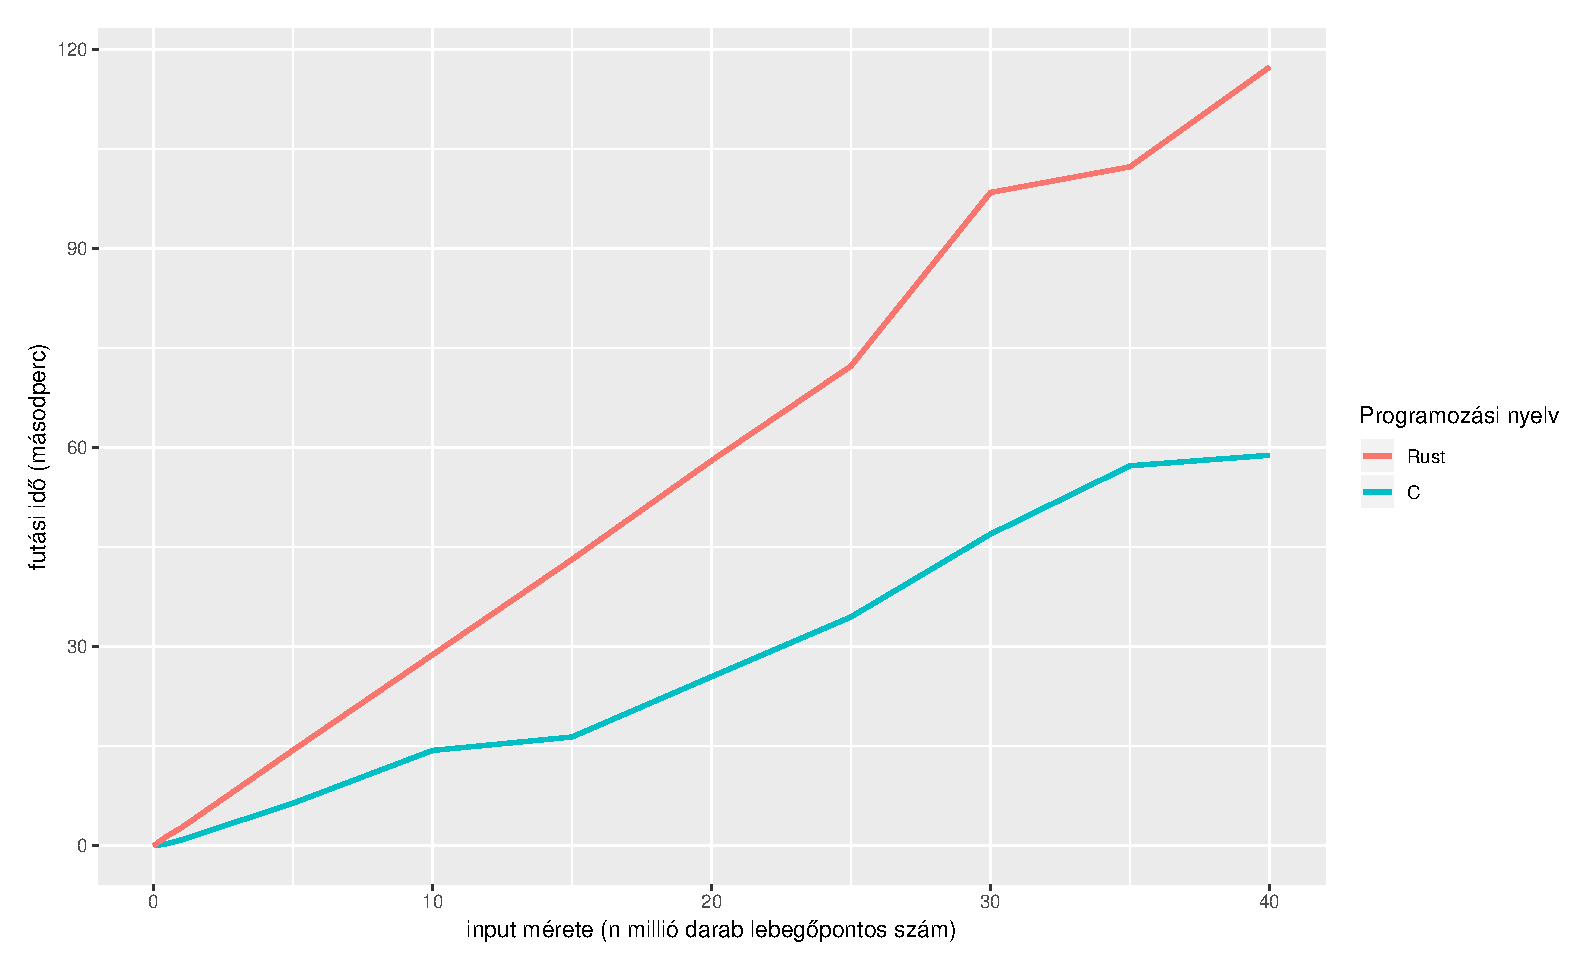
\includegraphics[width=15.5cm]{kepek/heap_run.eps}
Látható, hogy a kupac-rendezés módszerét tekintve a Rust nyelvű implementáció lassabb, mint a C-s megfelelője.

Kupac-rendezés maximális memóriafoglalása

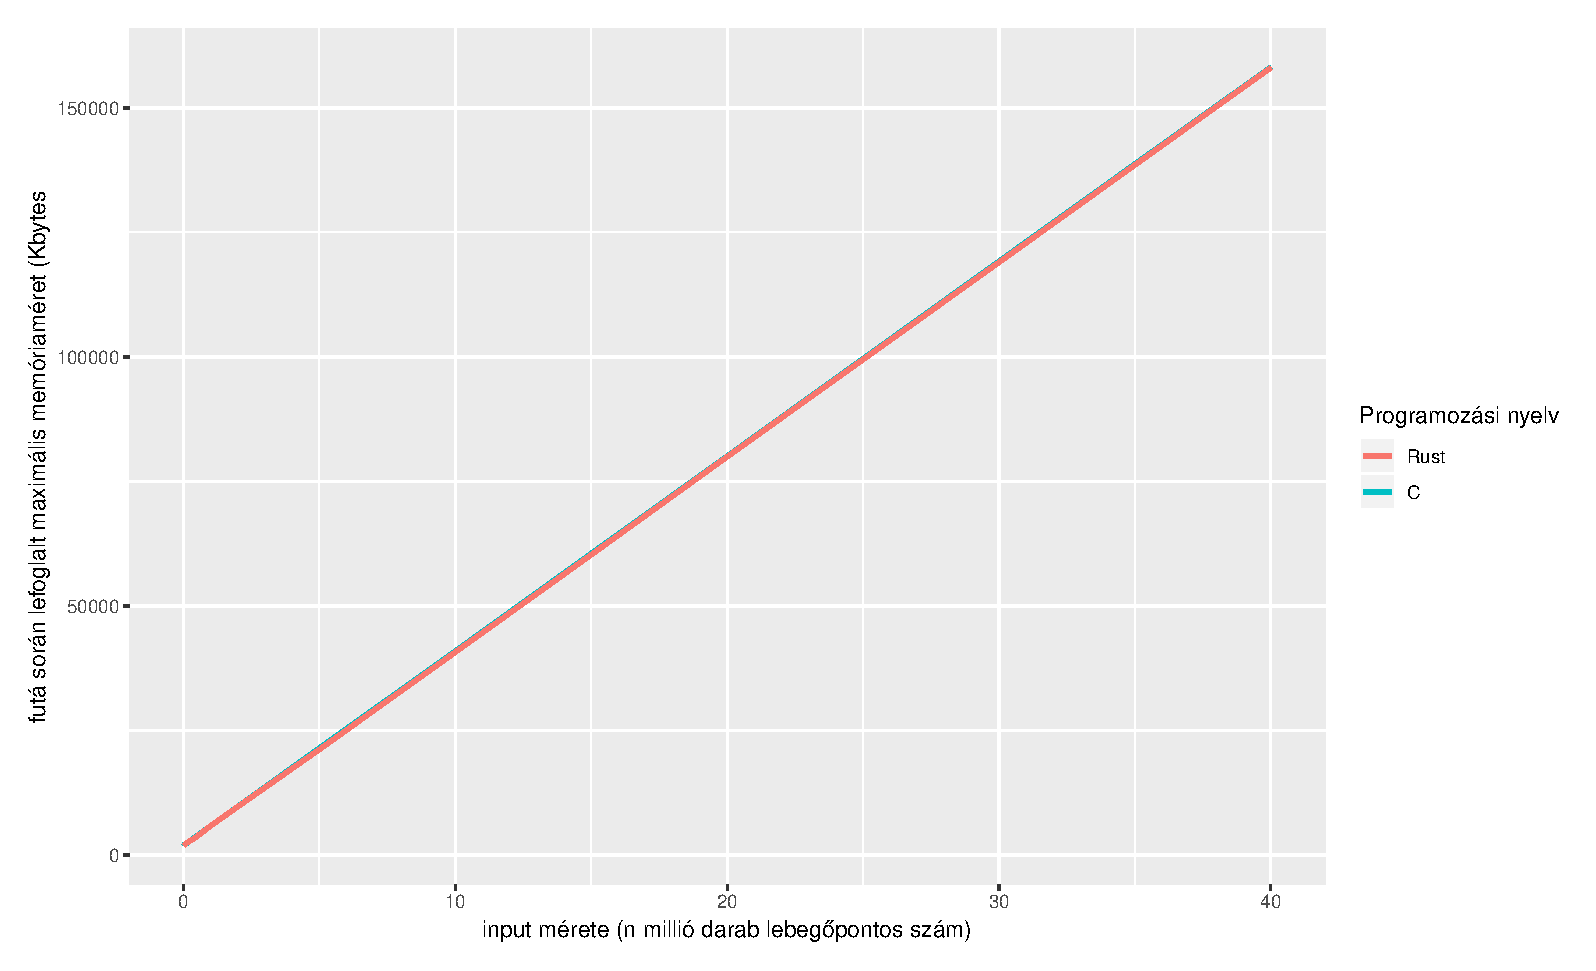
\includegraphics[width=15.5cm]{kepek/heap_memory.eps}
A Rust és C nyelven elkészített implementációk között a maximális memóriafoglalást tekintve nincsenek jelentős eltérések.

\subsection{Shell-rendezés}
\subsubsection{Rövid matematikai bevezetés}
\subsubsection{C nyelvű referencia-implementáció}
\cppstyle{\begin{lstlisting}[language=c++]
void shell_sort(unsigned n, Vec *a) {
    int gap = (n / 2);
    float temp;
    int j;

    while (gap > 0) {
        for (unsigned i = gap; i < n; i++) {
            temp = a->elements[i];
            
            j = i;
            while ( (j >= gap) && (a->elements[(j-gap)] > temp) ) {
                a->elements[j] = a->elements[(j-gap)];
                j -= gap;
            }
            a->elements[j] = temp;
        }
        gap /= 2;
    }
}
\end{lstlisting}}
\subsubsection{Az algoritmus egy implementációja Rustban}
\begin{lstlisting}[language=Rust]
pub fn shell_sort(n: i32, a: &mut Vec<f32>) {
	let mut gap: i32 =  (n / 2) as i32;
	let mut temp: f32;
	let mut j: i32;
	
	while gap > 0 {
		for i in gap..n {
			temp = a[i as usize];
			
			j = i;
			while j >= gap && a[(j-gap) as usize] > temp {
				a[j as usize] = a[(j-gap) as usize];
				j -= gap;
			}
			a[j as usize] = temp;
		}
		gap /= 2;
	}
}
\end{lstlisting}
\subsubsection{Futtatások eredményei}
Shell-rendezés futási ideje

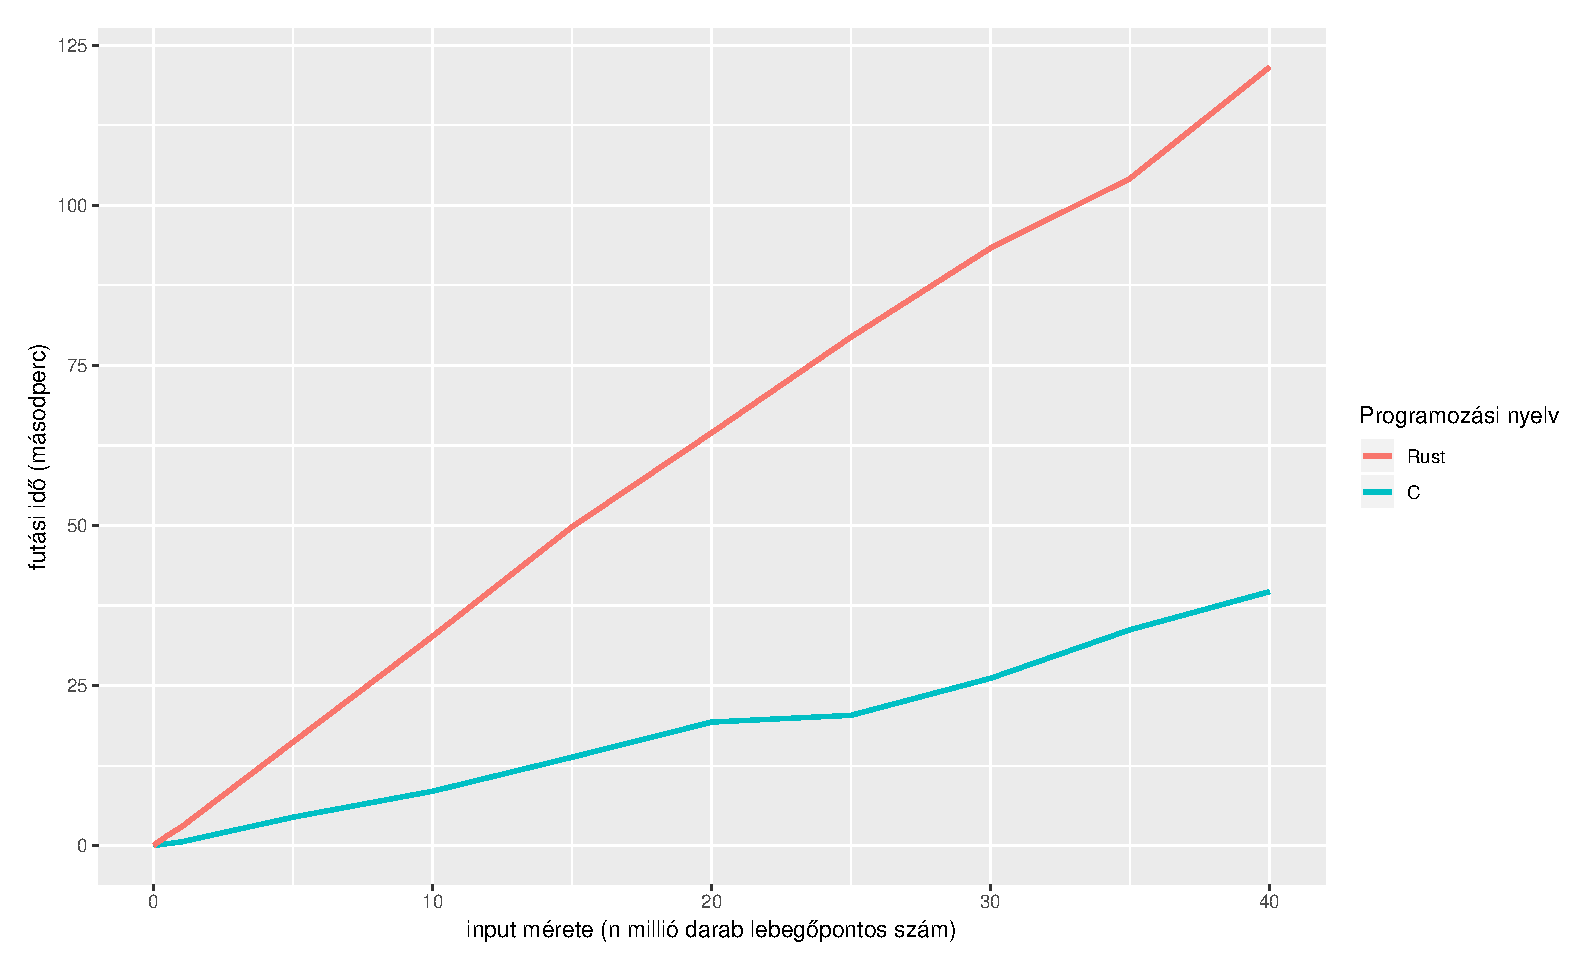
\includegraphics[width=15.5cm]{kepek/shell_run.eps}
Látható, hogy a Shell-rendezés módszerét tekintve a Rust nyelvű implementáció lassabb, mint a C-s megfelelője.

Shell-rendezés maximális memóriafoglalása

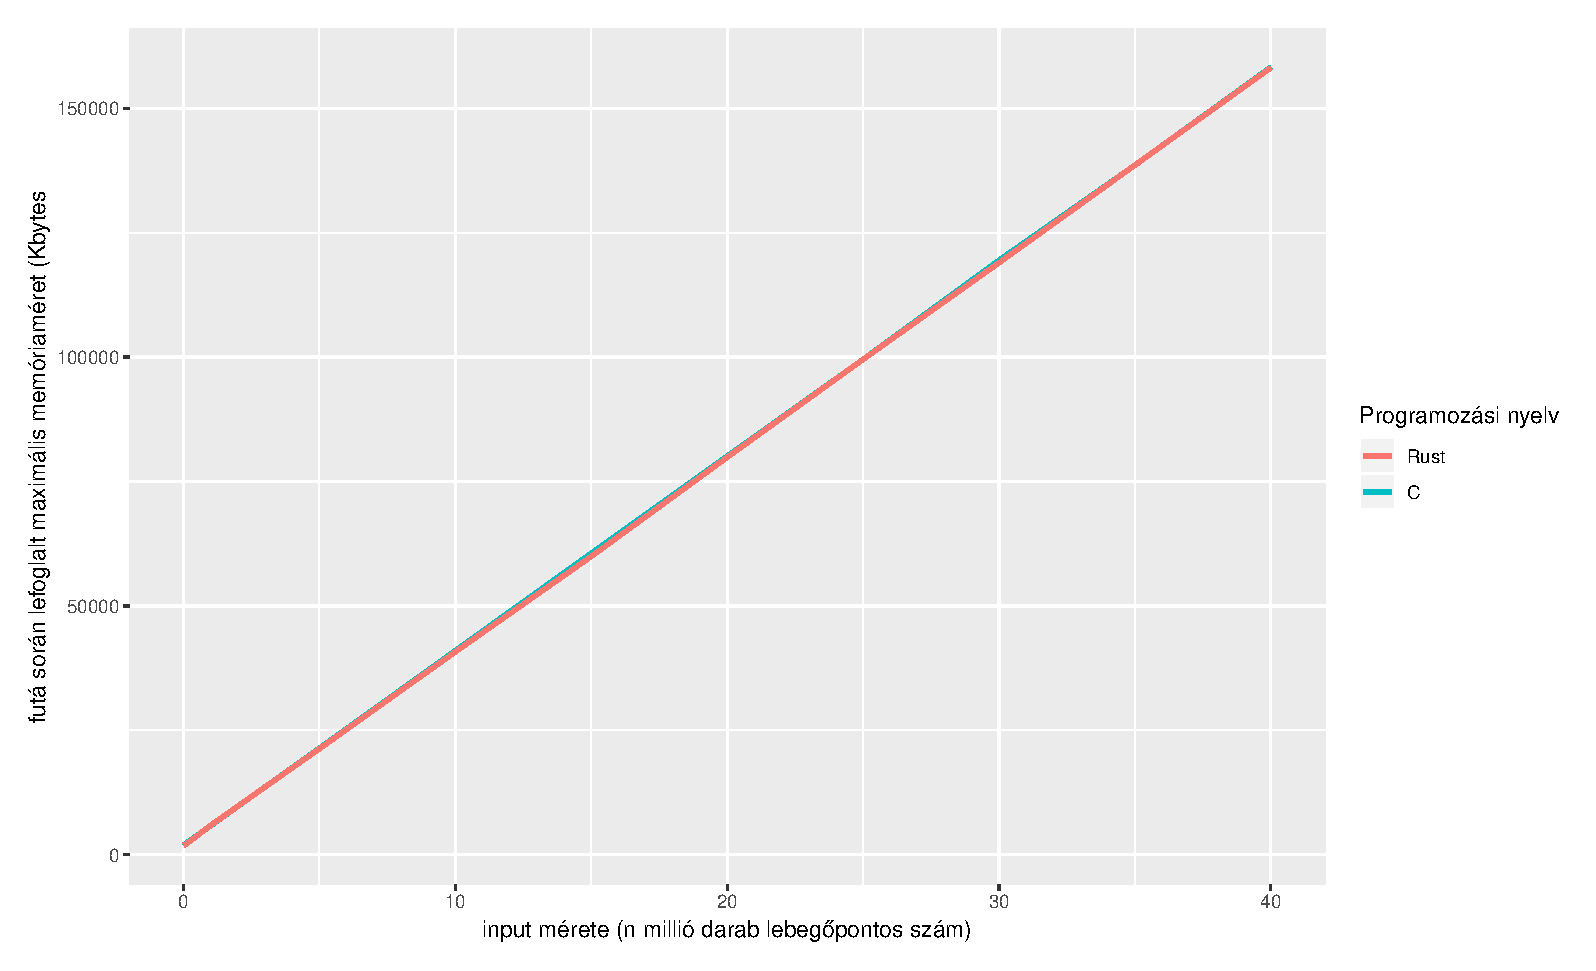
\includegraphics[width=15.5cm]{kepek/shell_memory.eps}
A Rust és C nyelven elkészített implementációk között a maximális memóriafoglalást tekintve nincsenek jelentős eltérések.

\subsection{Gyorsrendezés (Quicksort)}
\subsubsection{Rövid matematikai bevezetés}
\subsubsection{C nyelvű referencia-implementáció}
\cppstyle{\begin{lstlisting}[language=c++]
int partition(int low, int high, Vec *arr) {
    float pivot;

    int mid = (low + high) / 2;
    if (arr->elements[mid] < arr->elements[low]) {
        SWAP(float, arr->elements[low], arr->elements[high]);
    }

    if (arr->elements[high] < arr->elements[low]) {
        SWAP(float, arr->elements[low], arr->elements[high]);
    }

    if (arr->elements[mid] < arr->elements[high]) {
        SWAP(float, arr->elements[mid], arr->elements[high]);
    }

    pivot = arr->elements[high];

    int i;
    int j;

    i = low - 1;
	j = high + 1;

    while (1) {
        while (1) {
            i += 1;
            if (arr->elements[i] >= pivot) {
                break;
            }
        }

        while (1) {
            j -= 1;
            if (arr->elements[j] <= pivot) {
                break;
            }
        }

        if (i >= j) {
            return j;
        }

        SWAP(float, arr->elements[i], arr->elements[j]);
    }
}

void quicksort(int low, int high, Vec *arr) {
    if (low < high) {
        int p = partition(low, high, arr);
        quicksort(low, p, arr);
        quicksort(p+1, high, arr);
    } else {
        return;
    }
}
\end{lstlisting}}
\subsubsection{Az algoritmus egy implementációja Rustban}
\begin{lstlisting}[language=Rust]
pub fn quicksort(low: i32, high: i32, arr: &mut Vec<f32>) {
	if low < high {
		let p: i32 = partition(low, high, arr);
		quicksort(low, p, arr);
		quicksort(p+1, high, arr);
	} else {
		return;
	}
}

fn partition(low: i32, high: i32, arr: &mut Vec<f32>) -> i32 {
	let pivot: f32;

	let mid: i32 = (low + high) / 2;
	if arr[mid as usize] < arr[low as usize] {
		arr.swap(low as usize, high as usize);
	}
	if arr[high as usize] < arr[low as usize] {
		arr.swap(low as usize, high as usize);
	}
	if arr[mid as usize] < arr[high as usize] {
		arr.swap(mid as usize, high as usize);
	}
	pivot = arr[high as usize];

	let mut i: i32;
	let mut j: i32;

	i = low - 1;
	j = high + 1;

	loop {
		loop {
			i += 1;
			if arr[i as usize] >= pivot {
				break;
			}
		}

		loop {
			j -= 1;
			if arr[j as usize] <= pivot {
				break;
			}
		}

		if i >= j {
			return j as i32;
		}

		arr.swap(i as usize, j as usize);
	}
}
\end{lstlisting}
\subsubsection{Futtatások eredményei}
Gyorsrendezés futási ideje

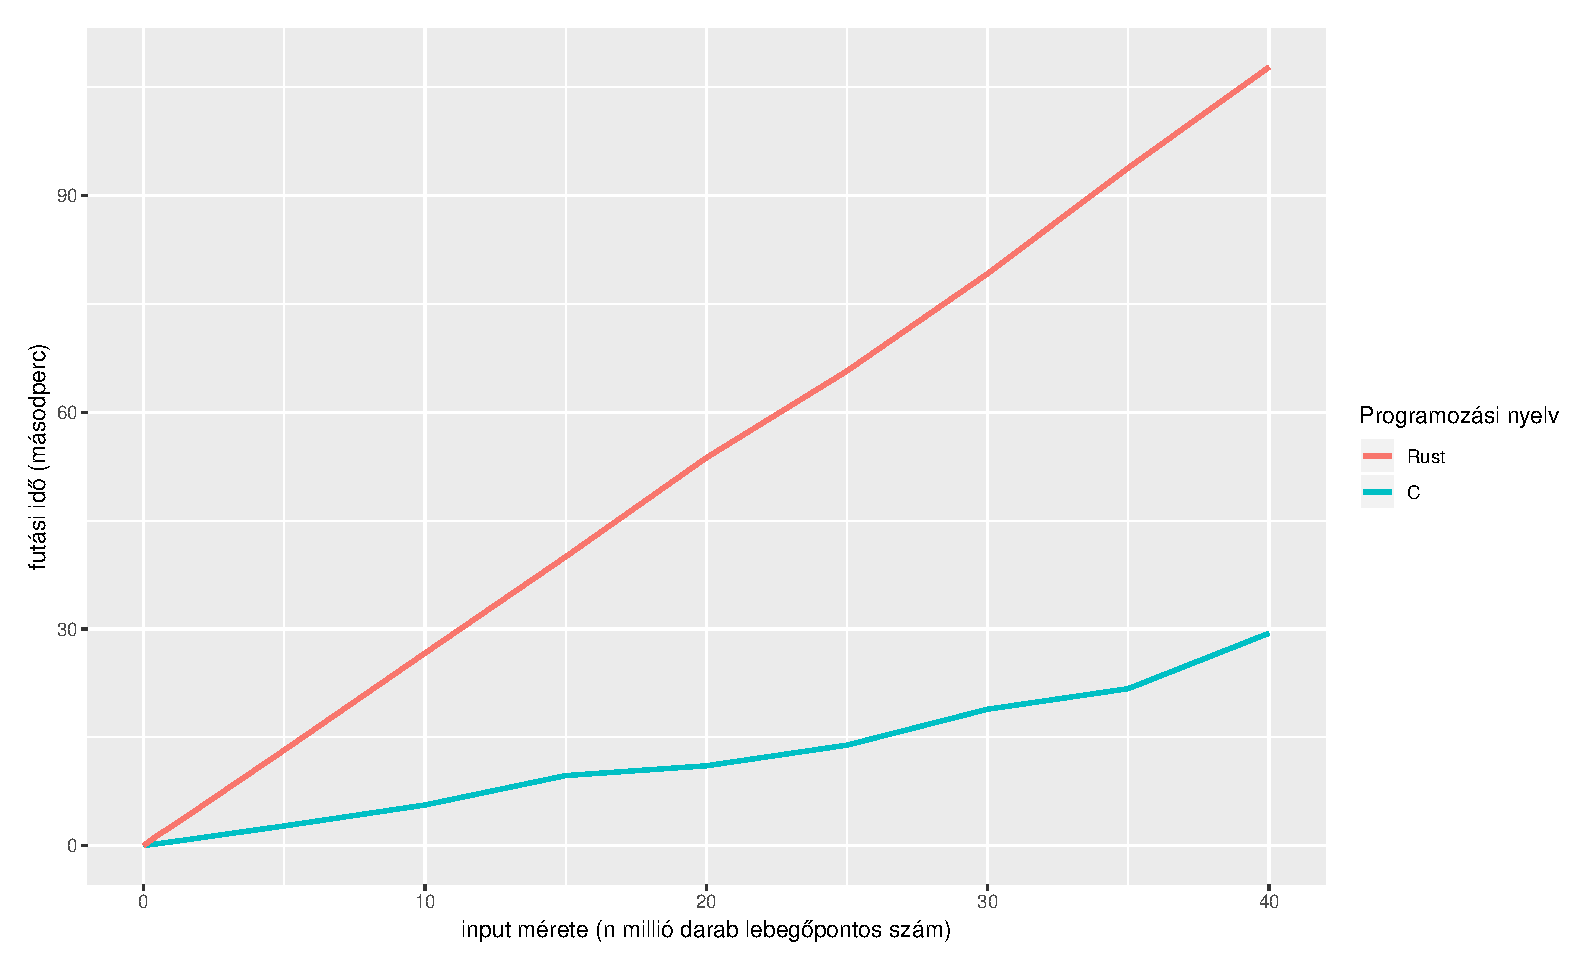
\includegraphics[width=15.5cm]{kepek/quick_run.eps}
Látható, hogy a gyorsrendezés módszerét tekintve a Rust nyelvű implementáció lassabb, mint a C-s megfelelője.

Gyorsrendezés maximális memóriafoglalása

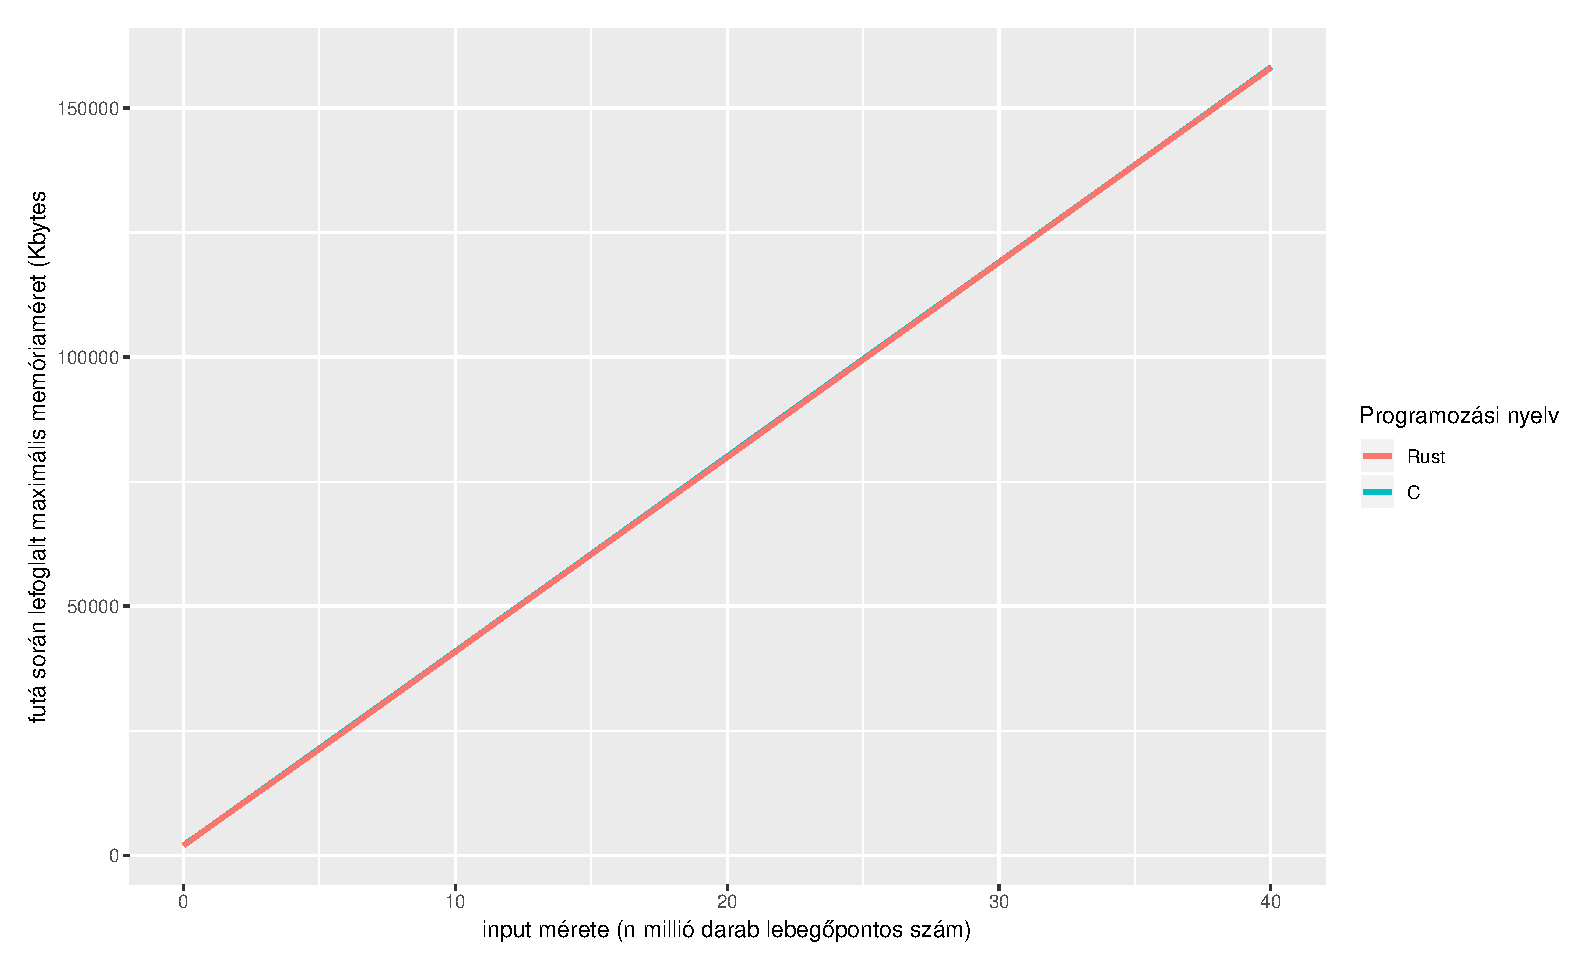
\includegraphics[width=15.5cm]{kepek/quick_memory.eps}
A Rust és C nyelven elkészített implementációk között a maximális memóriafoglalást tekintve nincsenek jelentős eltérések.

\section{Interpoláció}

\subsection{Lineáris interpoláció}
\subsubsection{Rövid matematikai bevezetés}
A lineáris interpoláció két ismert pont közötti összefüggést egyenes arányossággal közelíti. Az ismert pontok által meghatározott egyenesen lévő pontnak így elég az egyik koordinátáját ismerni a másik koordinátájának kiszámításához.
\[ y_n = \frac{x_n - x_1}{x_2 - x_1} * (y_2 - y_1) + y_1 \]
Ahol $x_1 \neq x_2$.
\subsubsection{C nyelvű referencia-implementáció}
\cppstyle{\begin{lstlisting}[language=c++]
float linear_interpolation(float x1, float y1, float x0, float y0, float x) {
    float delta;
    delta = x1 - x0;
    float y;

    if (delta == 0.0) {
        y = y0;
    } else {
        y = y0 + ( (x - x0) / delta) * y1;
    }

    return y;
}
\end{lstlisting}}
\subsubsection{Az algoritmus egy implementációja Rustban}
\begin{lstlisting}[language=Rust]
fn linear_interpolation(x1: f32, y1: f32, x0: f32, y0: f32, x: f32) -> f32 {
  let delta: f32;
  delta = x1 - x0;
  let y;

  if delta == 0.0 {
      y = y0;
  } else {
      y = y0 + ( (x - x0) / delta) * y1;
  }

  return y;
}
\end{lstlisting}
\subsubsection{Futtatások eredményei}
Lineáris interpoláció futási ideje

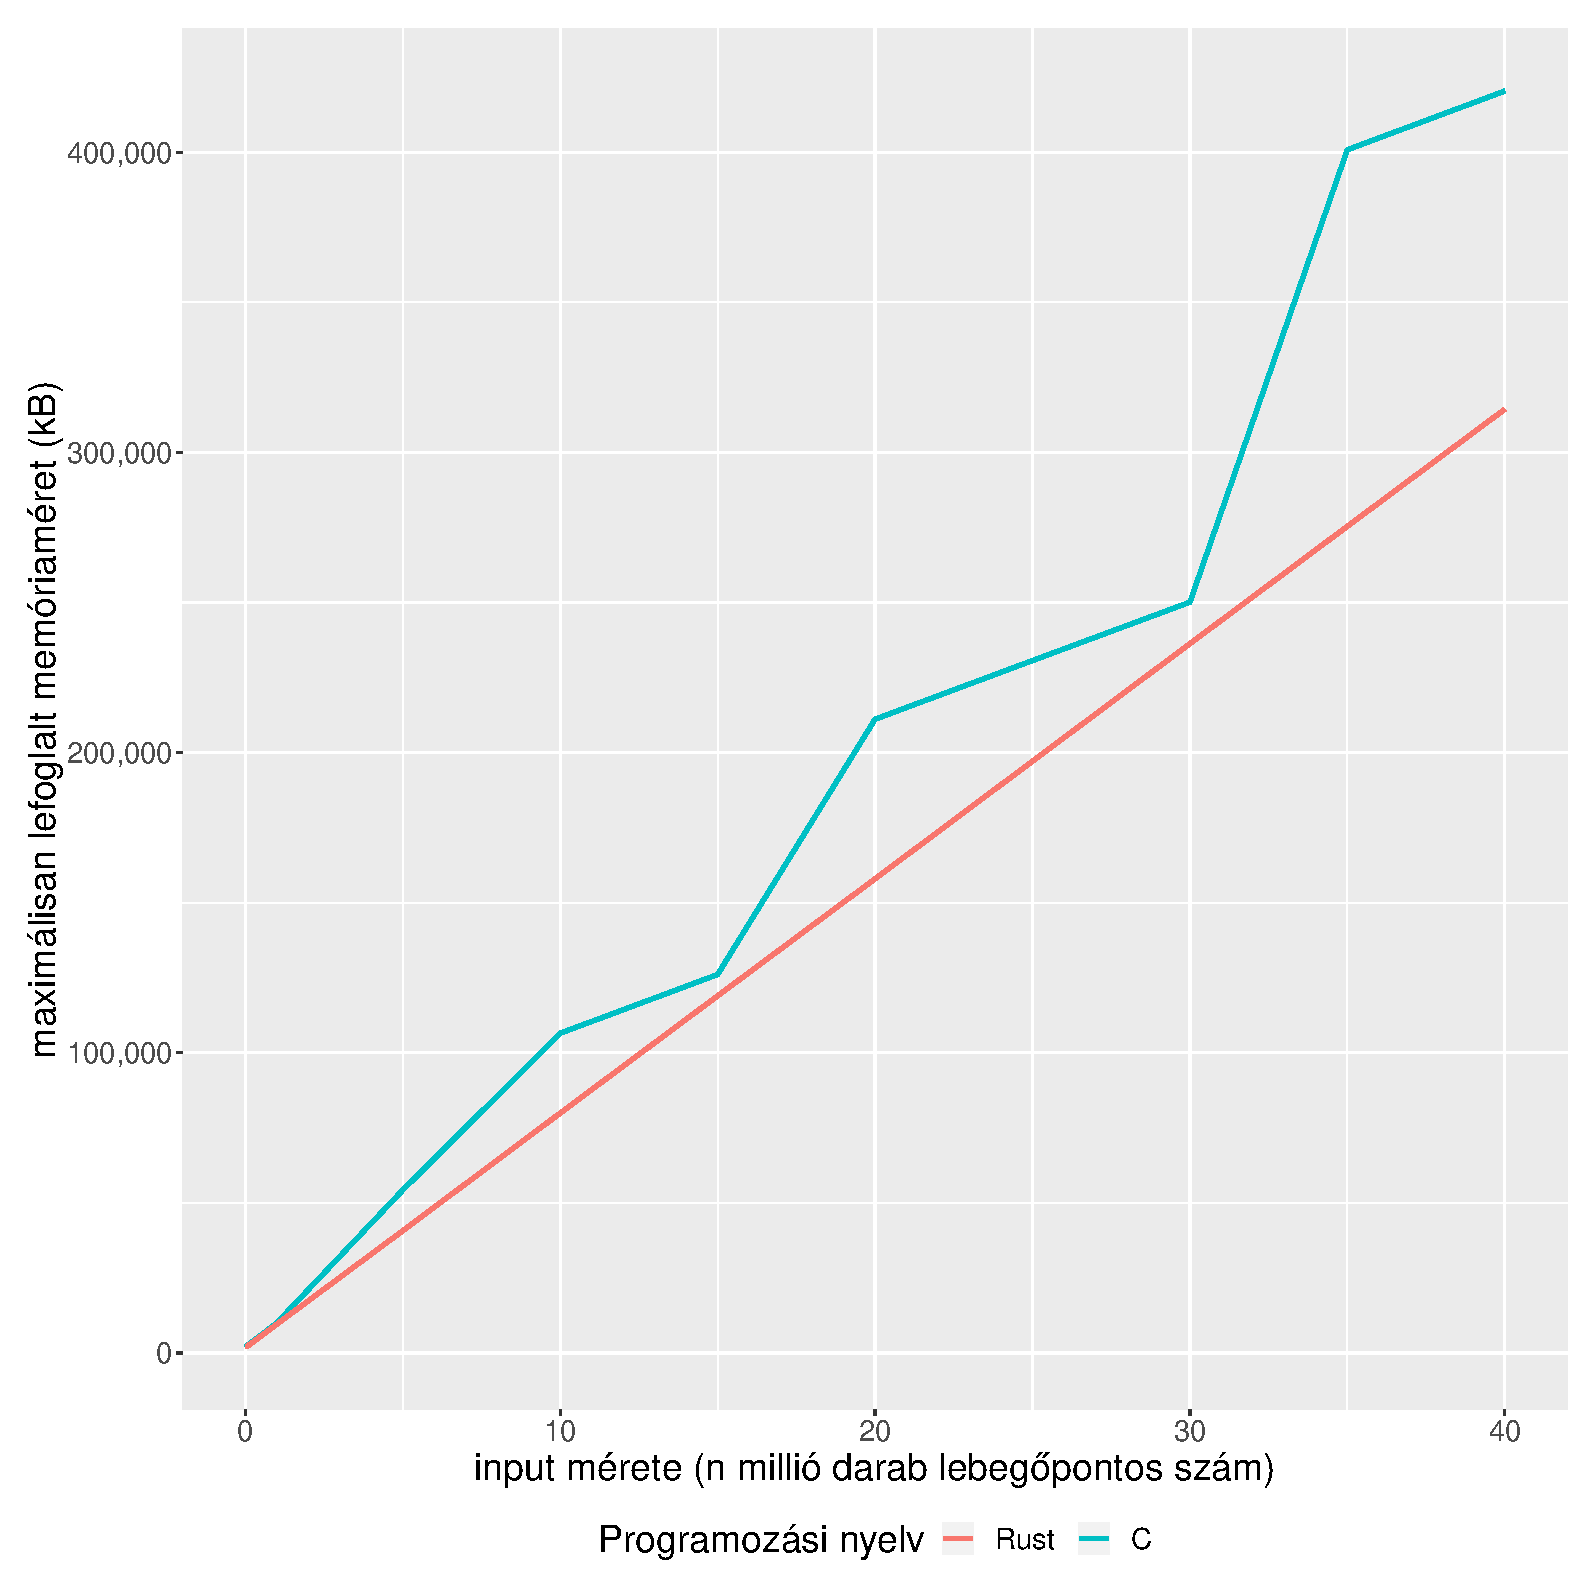
\includegraphics[width=15.5cm]{kepek/linear_interpolation_memory.eps}
Látható, hogy a lineáris interpoláció módszerét tekintve a Rust nyelvű implementáció lassabb, mint a C-s megfelelője.

Lineáris interpoláció maximális memóriafoglalása

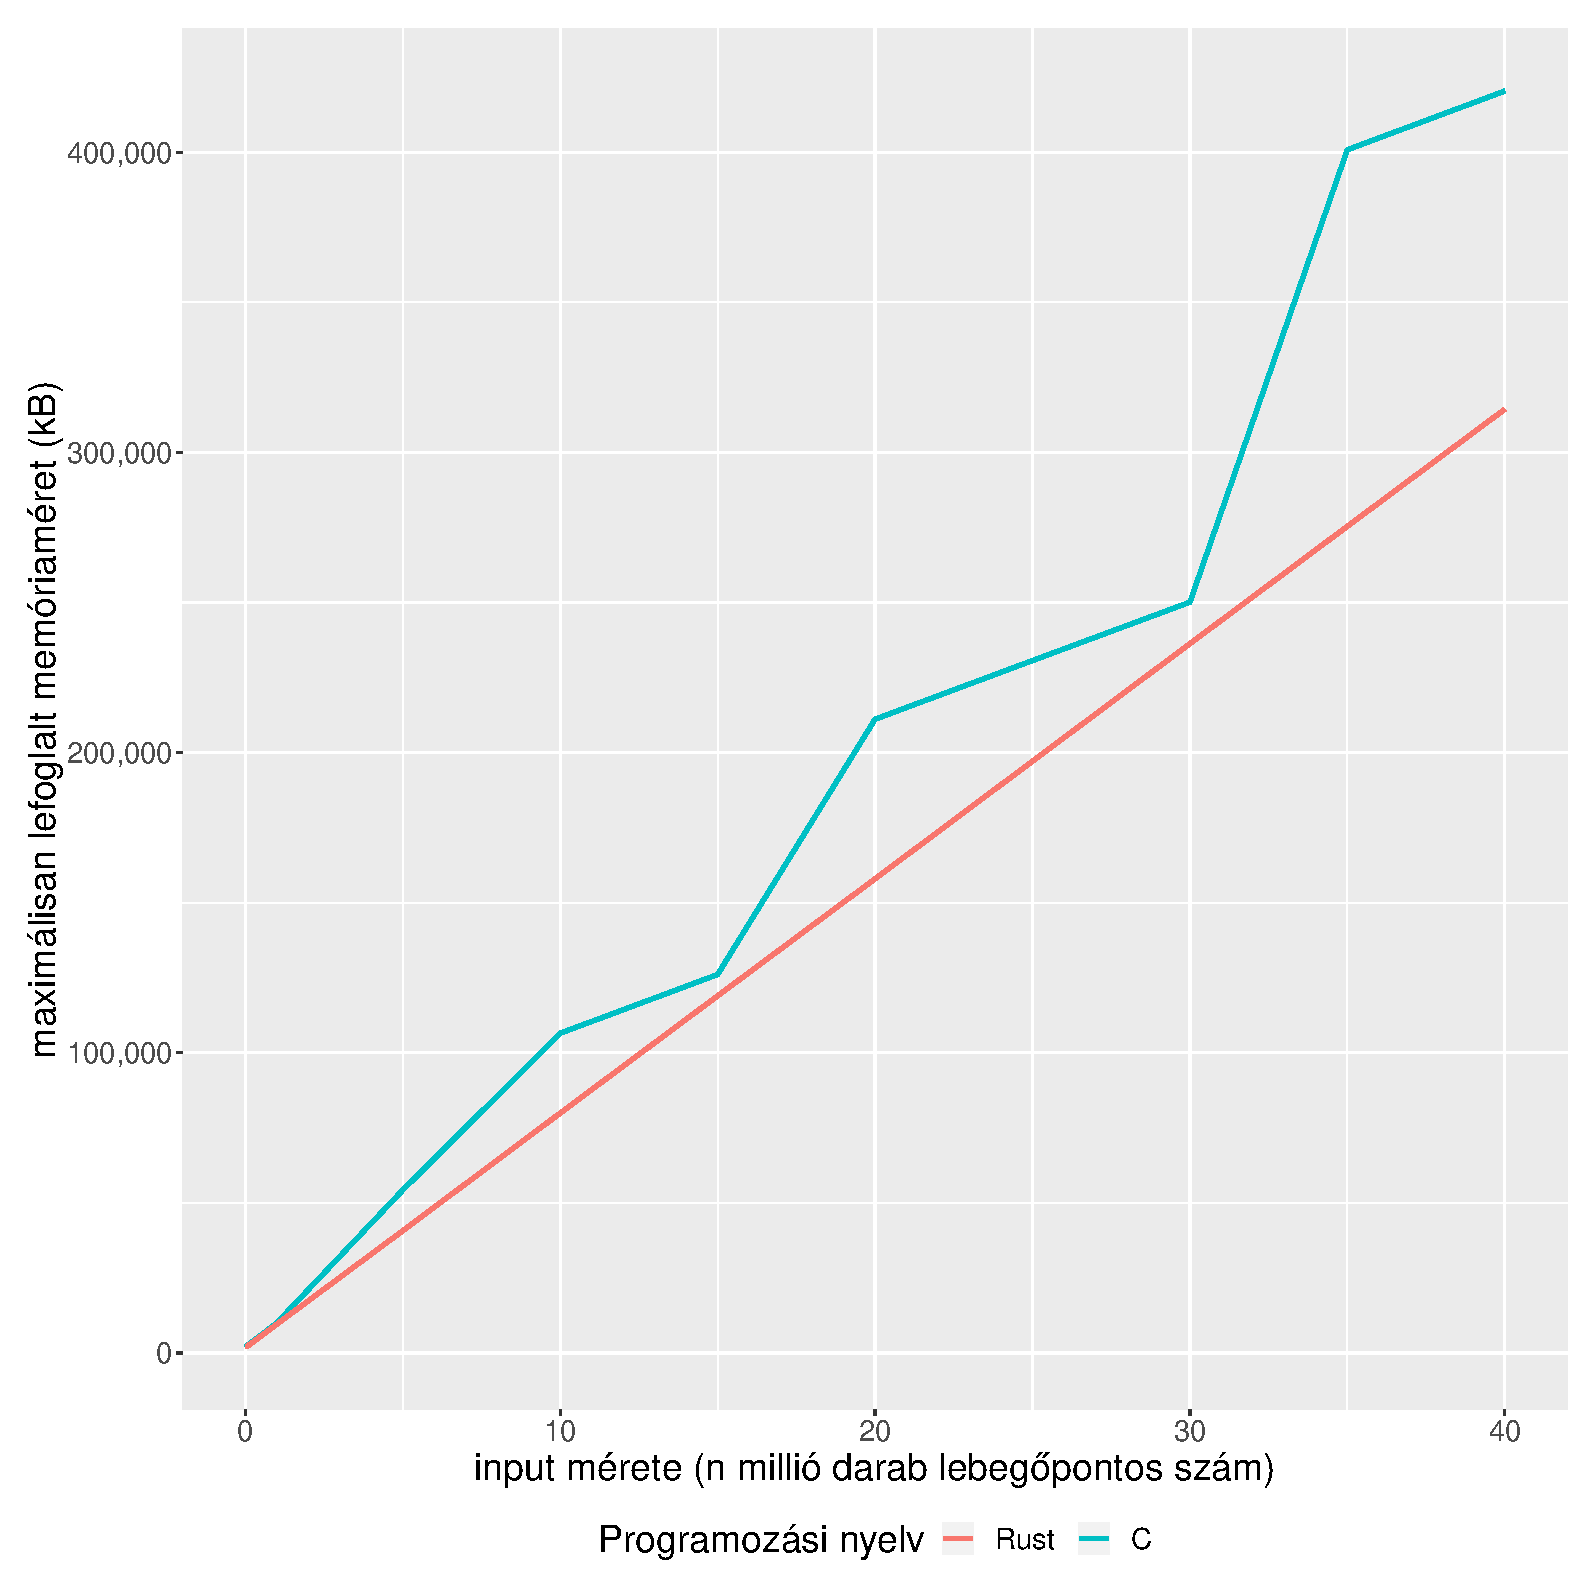
\includegraphics[width=15.5cm]{kepek/linear_interpolation_memory.eps}
A Rust és C nyelven elkészített implementációk között a maximális memóriafoglalást tekintve nincsenek jelentős eltérések.

\Chapter{Optimalizálás}

\section{Profilozás}
Azoknál a módszereknél, amelyek mért futásidejében jelentős különbség adódott a C-s, illetve a Rustos implementáció között van egy közös jellemzőjük: nagyméretű inputot olvasnak be fájlból. Így adódik a felvetés, hogy a fájl beolvasáshoz szükséges idő jelenti a differenciát a két implementáció között.

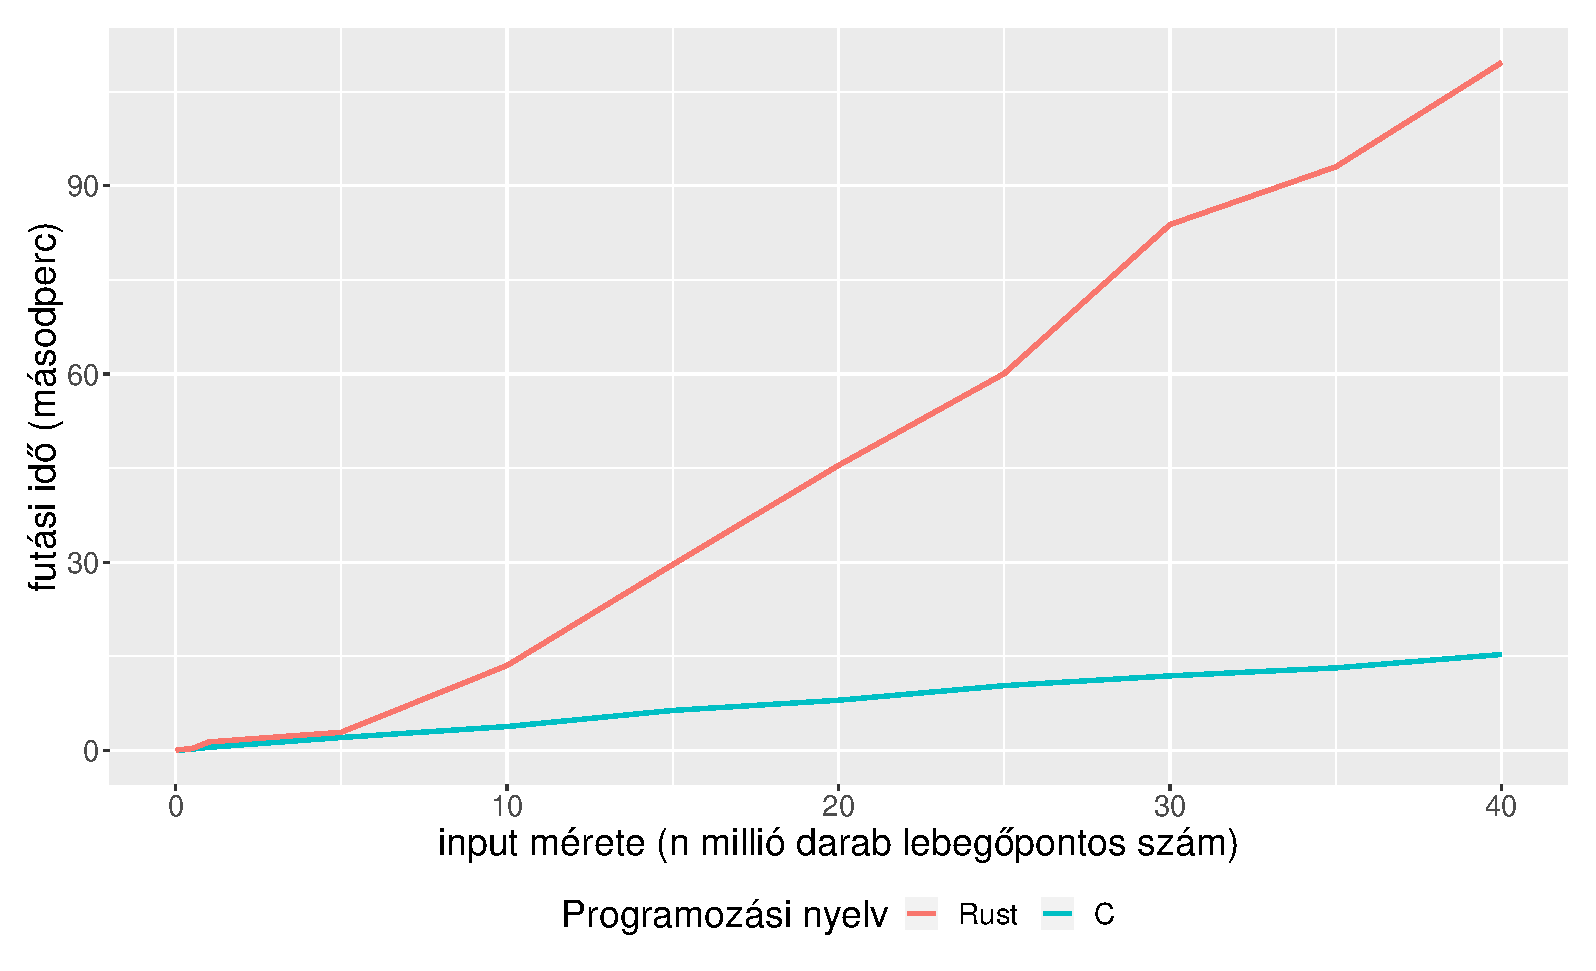
\includegraphics[width=15.5cm]{kepek/file_read.eps}
A grafikonon látható, hogy Rustban a beolvasás jóval lassabb, a futásidők különbségét magyarázza.
\subsection{Futásidők a fájl beolvasása nélkül}
\subsubsection{Kupacrendezés}
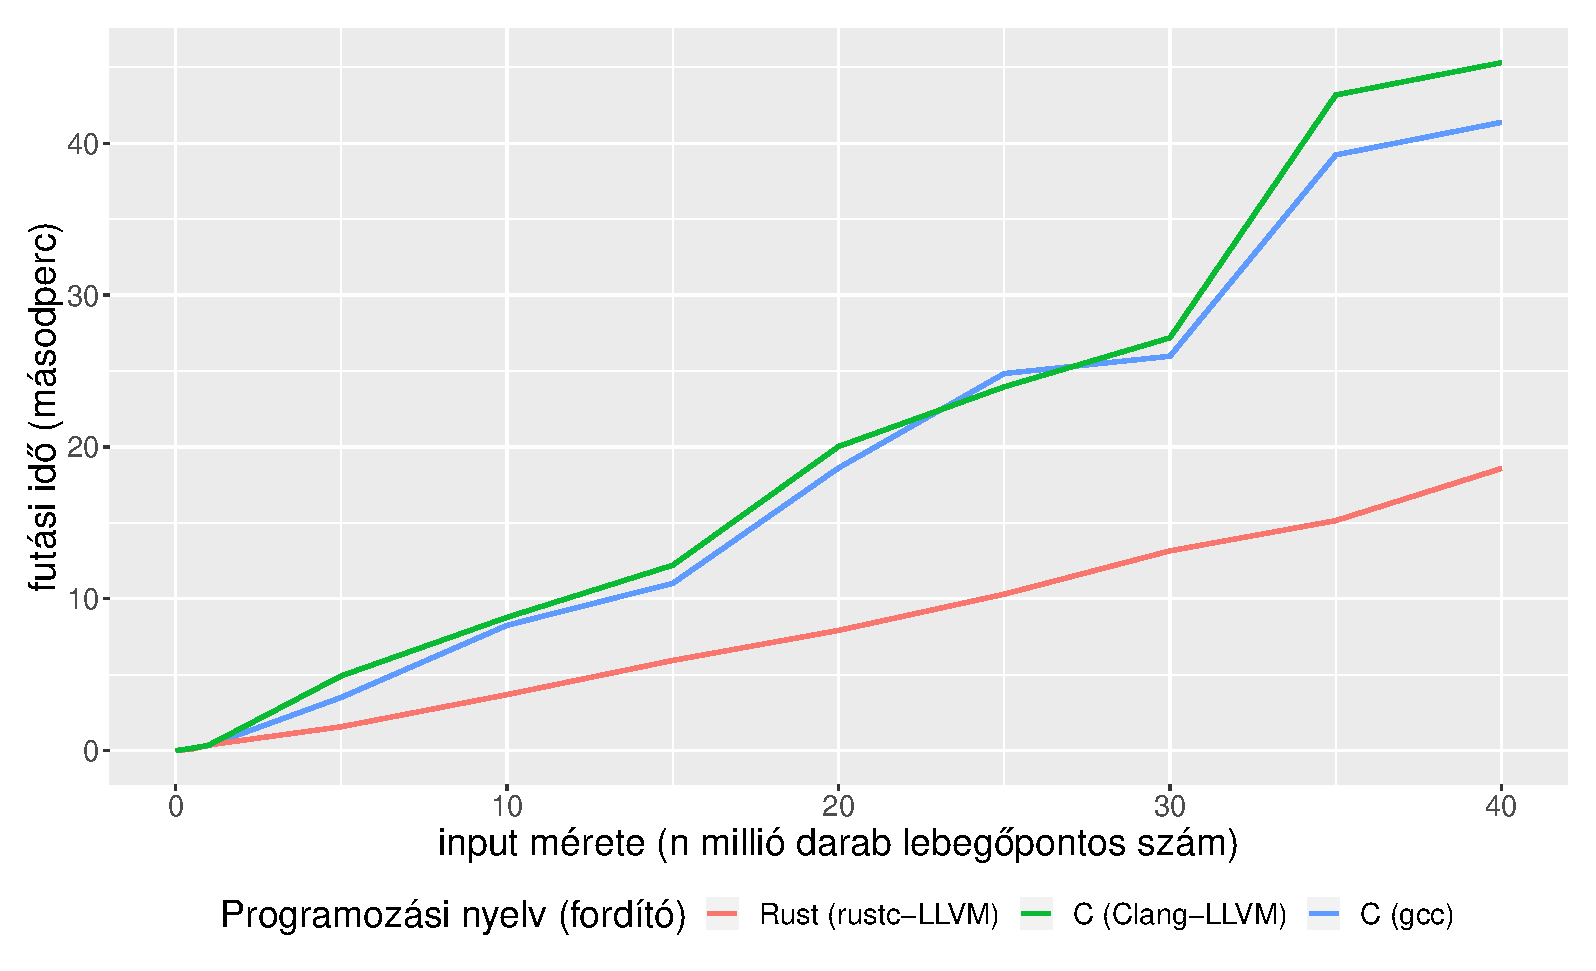
\includegraphics[width=15.5cm]{kepek/heap_sort_run_without_read.eps}
\subsubsection{Shell-rendezés}
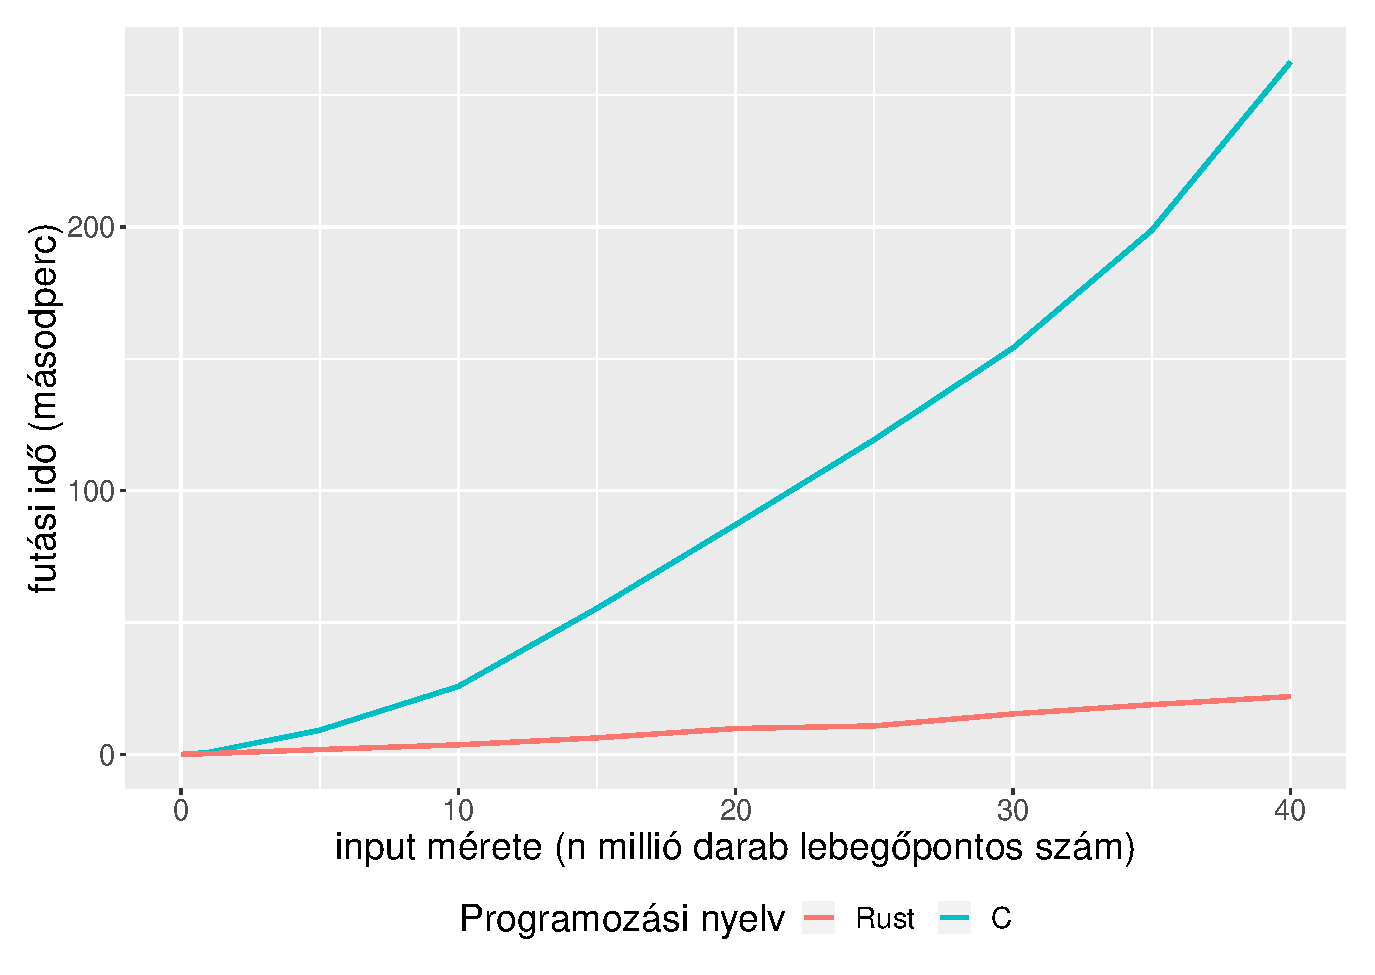
\includegraphics[width=15.5cm]{kepek/shells_sort_run_without_read.eps}
\subsubsection{Gyorsrendezés}
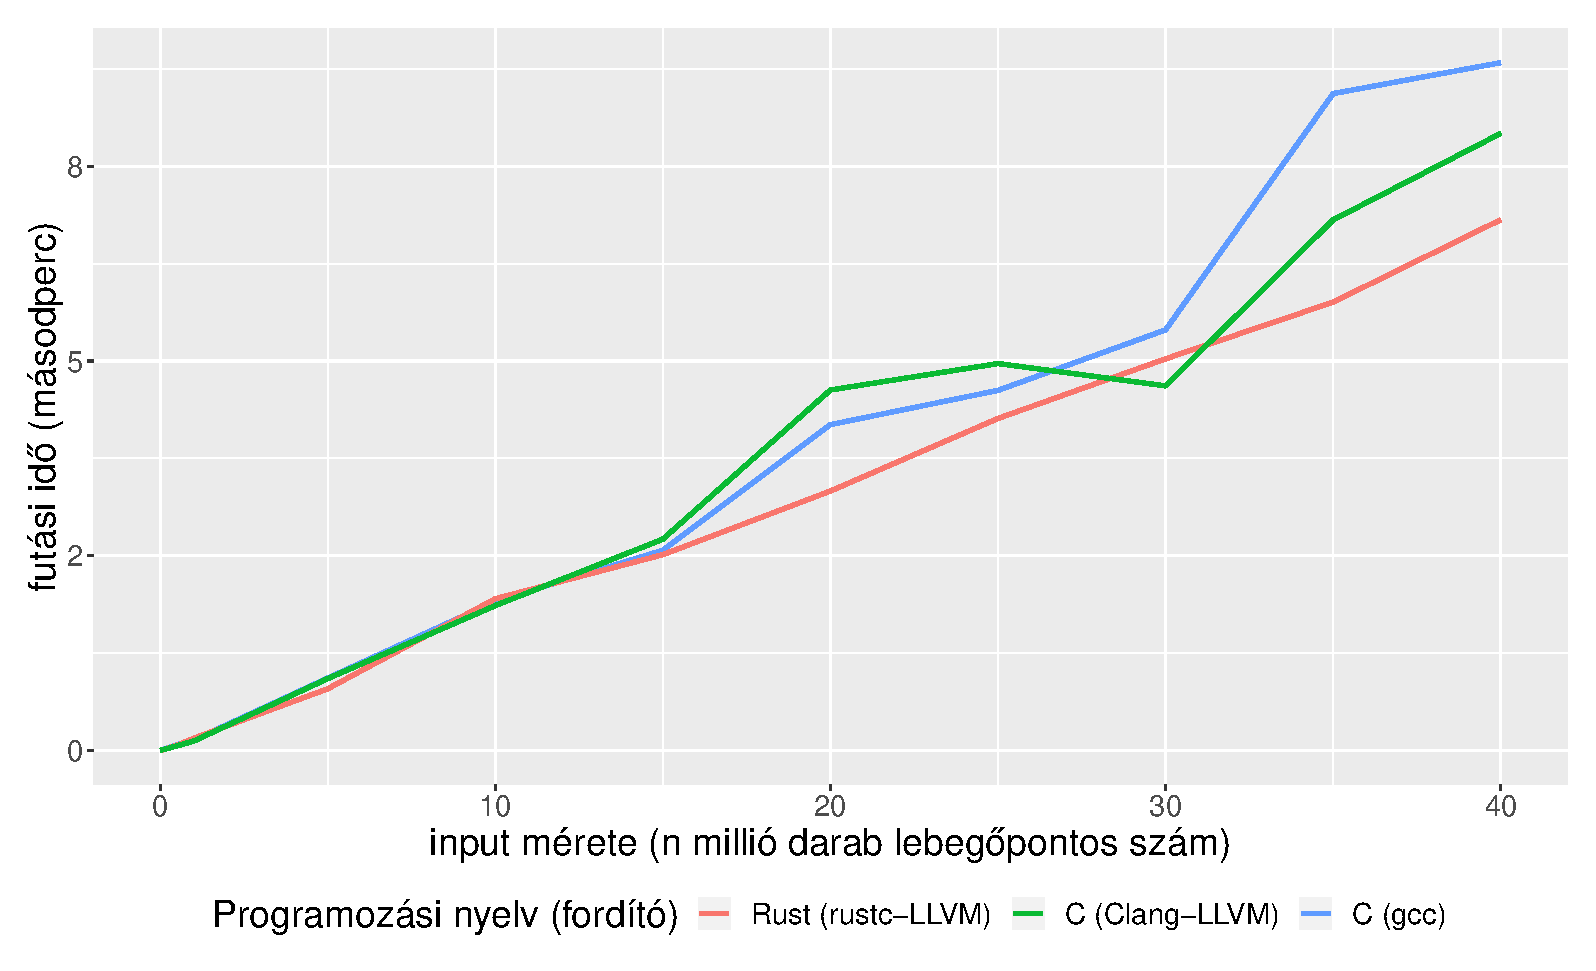
\includegraphics[width=15.5cm]{kepek/quicksort_run_without_read.eps}
\subsubsection{Lineáris interpoláció}
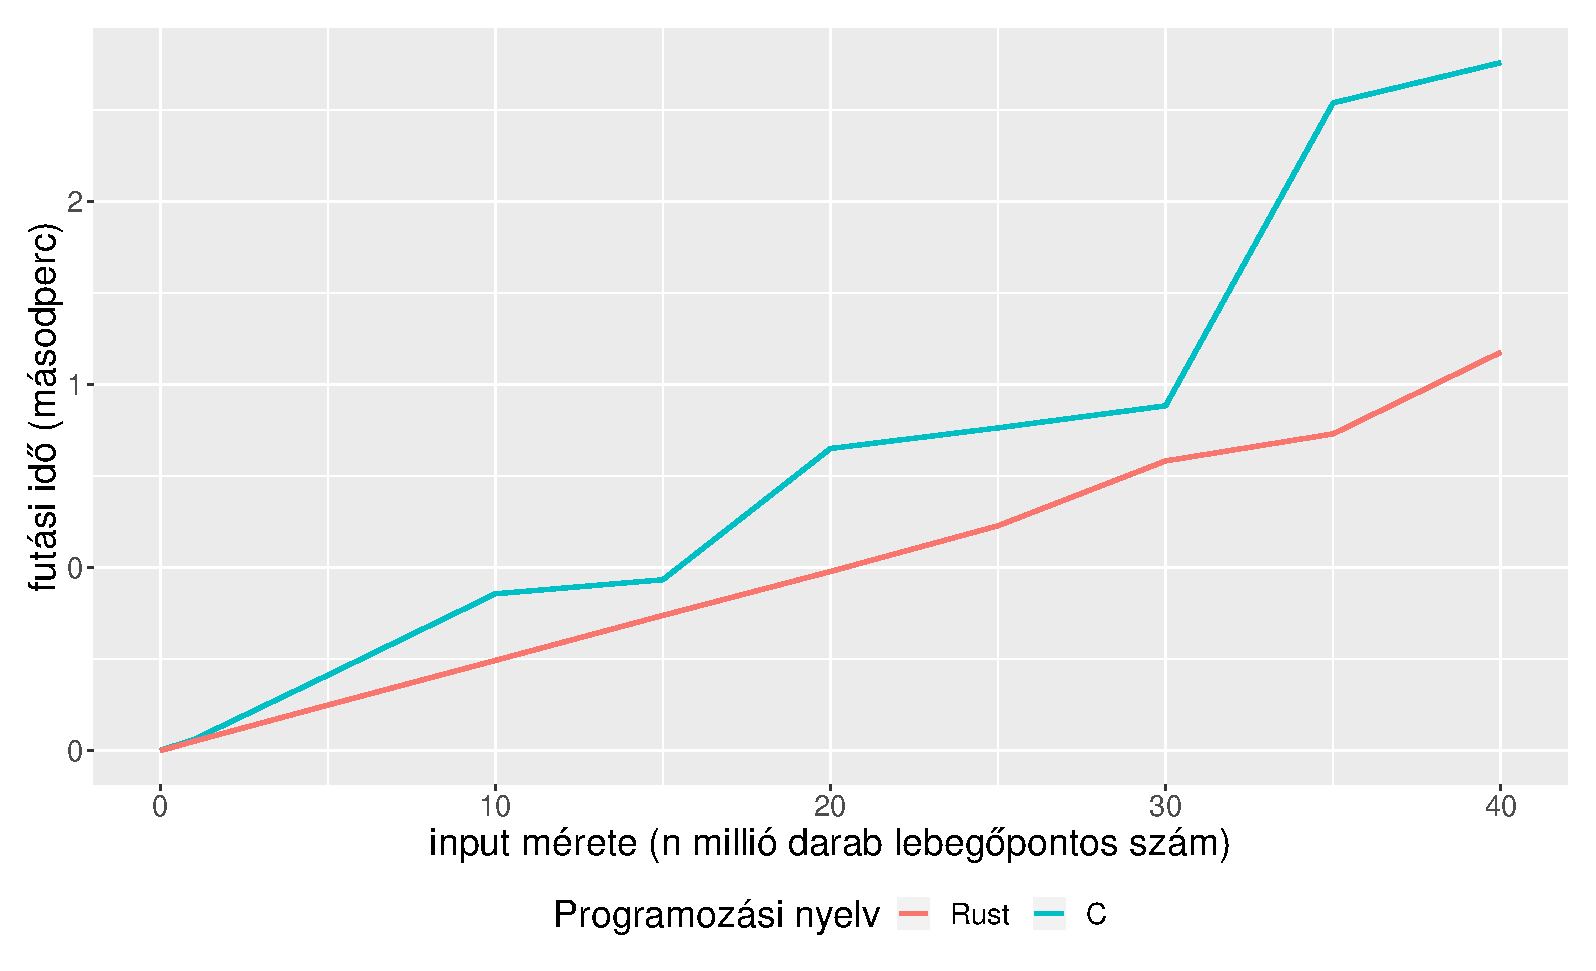
\includegraphics[width=15.5cm]{kepek/linear_interpolation_run_without_read.eps}
Látható, hogy maga a módszer a Rust implementációban minden esetben gyorsabb, ha az inputfájlok beolvasásást nem mérjük.

\section{Technikai részletek}
Lebegőpontos számok ábrázolását a Rust az IEEE-754-es szabványnak megfelelően végzni. Az egyszeres pontosságú lebegőpontos számokat az \lstinline{f32}, a dupla pontosságú lebegőpontos számokat pedig az \lstinline{f64} típusok szolgáltatják. C-ben ez nincs specifikálva, de általában az IEEE szabványát követi. Az egyszeres pontosságú a \lstinline{float}, a dupla pontosságú lebegőpontos szám a \lstinline{double} típussal reprezentálható.
%https://doc.rust-lang.org/book/ch03-02-data-types.html

A Rust nyelven implementált rendezési eljárások esetén a beépített \lstinline{Vec} adatszerkezetet használtam, melynek működéséhez hasonló saját típust definiáltam C-ben is. Ugyanakkor megemlítendő, hogy a C-s \lstinline{Vec} típus nem implementálja a Rustban meglévő vektortípus által implementált összes metódust, csak azt azokat, amelyek a dolgozatban bemutatott módszerek által használtak.
%https://doc.rust-lang.org/stable/nomicon/vec-alloc.html
\cppstyle{\begin{lstlisting}[language=c++]
typedef struct Vec {
  float *elements;
  size_t len;
  size_t capacity;
}

void vec_init(Vec *vec, size_t with_capacity) {
    vec->elements = (float*)malloc(with_capacity * sizeof(float) );
    vec->len = 0;
    vec->capacity = with_capacity;
}

void vec_insert(Vec *vec, float element) {
    if (vec->len == vec->capacity) {
        vec->capacity *= 2;
        vec->elements = (float *)realloc(vec->elements, vec->capacity * sizeof(float) );
    }
    vec->elements[vec->len++] = element;
}

Vec vec_copy(Vec *original_vec) {
    Vec new_vec;
    vec_init(&new_vec, original_vec->capacity);
    
    for (unsigned i = 0; i < original_vec->len; i++) {
        vec_insert(&new_vec, original_vec->elements[i]);
    }
    return new_vec;
}

void vec_free(Vec *vec) {
    free(vec->elements);
    vec->elements = NULL;
    vec->len = vec->capacity = 0;
}
\end{lstlisting}}

\section{Fordítóprogram-specifikus beállítások}
\subsection{A GNU GCC fordítóprogram specifikus beállításai (C)}
A C nyelvű implementációk fordításához a GNU GCC fordítóprogramot használtam, ami többféle optimalizálási lehetőséget is kínál. Alapértelmezetten, bármilyen opció megadása nélkül a fordító a fordítási időt próbálja minimalizálni.
\begin{itemize}
  \item Az \lstinline{-O1} opció bekapcsolja az összes olyan flaget, ami csökkentheti a kód méretét és a futási időt, anélkül, hogy a fordítási időt nagyban növelő opciót használna.
  \item Az \lstinline{-O2} opció bekapcsolja közel az összes olyan támogatott optimalizálási megoldást, ami nem jár együtt kompromisszumokkal a tárigény és a futási idő között. Tovább növeli a teljesítményt, viszont a fordítási idő is növekedhet az opció használatával.
  \item Az \lstinline{-O3} opció használ minden optimalizálást, amit az \lstinline{-O2} opció is, és még néhányat azon felül.
  \item Az \lstinline{-Ofast} opció futási sebességre optimalizál, használ minden optimalizálást, amit az \lstinline{-O3} kapcsoló is, ezeken felül pedig olyan optimalizálásokat is engedélyez, amelyek nem érvények minden szabványos programnak.
  \item Az \lstinline{-Os} opció a bináris méretére optimalizál. Használ minden optimalizálást, amit az \lstinline{-O2} opció is, kivéve azokat, amelyek sok esetben együtt járnak a tárigény növekedésével. Engedélyezi az \lstinline{-finline-funcions} kapcsolót, amely a fordítót a futási idő helyett a kódméret csökkentésére állítja. 
\end{itemize}
% https://gcc.gnu.org/onlinedocs/gcc/Optimize-Options.html
\subsection{A rustc fordítóprogram specifikus beállításai (Rust)}
\begin{itemize}
  \item A \lstinline{-C} vagy \lstinline{--codegen OPT[=VALUE]} opció használata esetén az \lstinline{opt-level} kapcsolóval állítható a fordító által alkalmazott optimalizálás szintje. A szint egyrészt 0-3 közötti egész szám lehet, ahol a 3 jelenti a leginkább optimalizált kimenetet. Az \lstinline{s} és \lstinline{z} szintek a fordítás során létrejövő bináris méretére optimalizál.
  \item Az \lstinline{-O} opció ekvivalens a \lstinline{-C opt-level=2} használatával.
\end{itemize}

\Chapter{Összegzés}
A dolgozatom alapján belátható, hogy a Rust programozási nyelvként egy ígéretes kezdeményezés, ami a teljesítményt illetően összehasonlítható a hasonló okból megbecsült C/C++ nyelvekkel. A nem is feltétlenül egyedi, de jól átgondolt nyelvi elemeinek köszönhetően a legtöbb hiba fordításidőben kiderül, ami nagy segítség a Rust nyelven programozók számára.

A rendszerprogramozás mellett a webfejlesztés, és a játékprogram-fejlesztés területe mellet már operációs rendszert is fejlesztenek vele.

Népszerűsége egyre növekszik a programozók körében, azonban a Rust ökoszisztémája továbbra is nélkülözi a kifinomult fejlesztői eszközöket. Integrált fejlesztői környezet a dolgozat írásakor még nem létezik olyan minőségben, mint a régebbi programozási nyelvekhez, mint például a C, C++, C\# vagy Java esetében.

Azonban hasznos tulajdonságai mellett sem elhanyagolható tény, hogy még mindig nem egy kiforrott nyelv. Látható, hogy a fájlbeolvasás a szabványos függvénykönyvtárbeli eszközökkel nagyon lassú a C-hez képest. A futási idők mérésénél például egy olyan esettel találkoztam, hogy a \lstinline{Duration} struktúrához több olyan metódus is létezik, amely az időtartam numerikus értékének kinyerésére szolgál. A mérések céljából a leginkább hasznosnak vélt \lstinline{as_float_secs} metódus, amely a másodperceket törtrészükkel együtt adja vissza, csak a \lstinline{nightly} API-val érhető el, ellenben a nanoszekundumokat, mikroszekundumokat visszaadó metódusok már a stabil API részei.
%https://doc.rust-lang.org/std/time/struct.Duration.html#method.as_float_secs

Ezen kívül vannak olyan be nem mutatott potenciáljai a Rust nyelvnek, amely a szakdolgozatnak nem témája. Ilyen például a viszonylag egyszerűen kezelhető párhuzamosság, amellyel tovább javítható a teljesítmény.

A numerikus módszerek implementálása Rustban összességében nem körülményesebb feladat, mint C-ben. Az ebben a dolgozatban bemutatott módszerek esetén az alapértelmezetten immutable változókra, az ownership-szabályokra, illetve a határozottan előjel nélküli (\lstinline{usize}) egész indexekre kellett a leginkább figyelni. Ezeken a nyelvi jellemzőkön kívül az elkészült forráskód hasonló a C-s megfelelőjéhez. Bemutatásra kerültek rendezési, numerikus integrálást és lineáris interpolációt megvalósító függvények.

Megjegyzendő, hogy vannak már olyan numerikus számításokra alkalmazható könyvtárak Rusthoz, amelyek jóval túlmutatnak a szakdolgozatomban bemutatott függvény-gyűjteményen, mint például a Peroxide. %https://crates.io/crates/peroxide

Ellenben jelenleg nem érhető el olyan széleskörű funkcionalitást nyújtó, és relatíve egyszerűen használható függvénykönyvtár numerikus problémákra, mint például az R, vagy a Python nyelvekhez.

A teljesítménymérések után megállapítható, hogy az eddig teljesítménykritikus problémák esetén gyakran alkalmazott C/C++ nyelvekhez hasonló, nem ritkán még jobb teljesítmény érhető el a Rust segítéségével. Az ownership-szabályok mentén meghatározott memóriakezelés egyrészt biztosítja, hogy nincs futásidőben szükség garbage collectorra, így a Rust nyelvű implementációk memóriafoglalása nem tér el jelentősen a C-s megvalósításokétól. Másrészt, lehetetlenné teszi az olyan memóriahibák létrehozását, mint a dangling pointer, vagy a duplán felszabadított memóriaterület. A fordításkor létrejövő bináris állományok terén a \lstinline{rustc} fordító még mindig nagyobb méretet eredményez, mint a már 8 főverziót megért \lstinline{gcc} fordítóprogram a C esetében.

Összefoglalva megállapítható, hogy a Rust alkalmas általános célú programozási nyelvnek, teljesítményre és memóriabiztonságra egyszerre fókuszáló rendszerprogramozási nyelvnek. Így numerikus módszerek számítógépi megvalósítására is, amelyekhez kiváló teljesítménymutatóival járul hozzá.


% !TEX encoding = UTF-8 Unicode

\begin{thebibliography}{x}
\addcontentsline{toc}{chapter}{\bibname}

% WARN: Ezek itt csak példaként szerepelnek!

\bibitem{artistic}
Papari, Giuseppe, Nicolai Petkov, and Patrizio Campisi. \emph{Artistic edge and corner enhancing smoothing}. IEEE Transactions on Image Processing 16.10 (2007): 2449-2462.

\bibitem{intellipaint}
Reese, L. Jack, and William A. Barrett. \emph{Image editing with intelligent paint}. Proceedings of Eurographics. Vol. 21. No. 3. 2002.

\bibitem{instagram}
Instagram, hivatalos weboldal, \texttt{https://www.instagram.com/}, Internet, 2018.

\bibitem{snapchat}
Snapchat, hivatalos weboldal, \texttt{https://www.snapchat.com/}, Internet, 2018.

\bibitem{messenger}
Facebook messenger, hivatalos weboldal, \texttt{https://www.messenger.com/features}, Internet, 2018.

\bibitem{prisma}
Prisma, hivatalos weboldal, \texttt{https://prisma-ai.com/}, Internet, 2018.

\bibitem{pixect}
Pixect, hivatalos weboldal, \texttt{https://www.pixect.com/}, Internet, 2018.

\bibitem{jetset}
Smilebit: \emph{Jet Set Radio}, SEGA, \texttt{http://www.sega.com/games/jet-set-radio}, Internet, 2003.

\bibitem{scannerdarkly}
The New York Times, \emph{'A Scanner Darkly': Keanu Reeves, Undercover and Flying High on a Paranoid Head Trip}, 2006. július 7.

\bibitem{porthu}
Port.hu, \emph{Kamera által homályosan}, \texttt{https://port.hu/adatlap/film/tv/kamera-altal-\\homalyosan-a-scanner-darkly/movie-82437}, Internet, 2006.

\bibitem{czap}
Czap László: Képfeldolgozás, egyetemi jegyzet, Miskolci Egyetem, \\ \texttt{http://mazsola.iit.uni-miskolc.hu/~czap/HEFOP/Kepfeld1010.pdf}, 2007.

\bibitem{kato}
Kató Zoltán: Digitális képfeldolgozás, egyetemi kurzus, Szegedi Tudományegyetem, \texttt{http://www.inf.u-szeged.hu/~kato/teaching/DigitalisKepfeldolgozasTG}, 2014.

\bibitem{bilateral}
Paris, Sylvain, et al. \emph{A gentle introduction to bilateral filtering and its applications}. ACM SIGGRAPH 2007 courses. ACM, 2007.

\bibitem{sobel}
Utkarsh Sinha: \emph{The Sobel and Laplacian Edge Detectors}, \texttt{http://aishack.in/tutorials/sobel-laplacian-edge-detectors/}, 2010.

\bibitem{beyeler} Michael Beyeler: \emph{How to create a cool cartoon effect with OpenCV and Python}, \texttt{http://www.askaswiss.com/2016/01/} \texttt{how-to-create-cartoon-effect-opencv-python.html}, 2016. január 5.

\bibitem{beyeler2} Michael Beyeler: \emph{How to create a beautiful pencil sketch effect with OpenCV and Python}, \texttt{http://www.askaswiss.com/2016/01/} \texttt{how-to-create-pencil-sketch-opencv-python.html}, 2016. január 13.

\bibitem{emami} Shervin Emami: \emph{Mastering OpenCV with Practical Computer Vision Projects}, Packt Publishing, 2012.

\bibitem{opencv}
Bradski, Gary, and Adrian Kaehler. Learning OpenCV: \emph{Computer vision with the OpenCV library}. O'Reilly Media, Inc., 2008.

% TODO: Artistic filter-es könyv.

\end{thebibliography}


% !TEX encoding = UTF-8 Unicode
\newpage
\section*{CD-melléklet tartalma}

A dolgozat PDF változatát a \texttt{dolgozat.pdf} fájlban találjuk.

A dolgozat \LaTeX\ segítségével készült. A forrásfájlok a \texttt{dolgozat} jegyzékben találhatók.

\[
\ldots
\]



\end{document}
